\documentclass[twoside]{book}

% Packages required by doxygen
\usepackage{fixltx2e}
\usepackage{calc}
\usepackage{doxygen}
\usepackage[export]{adjustbox} % also loads graphicx
\usepackage{graphicx}
\usepackage[utf8]{inputenc}
\usepackage{makeidx}
\usepackage{multicol}
\usepackage{multirow}
\PassOptionsToPackage{warn}{textcomp}
\usepackage{textcomp}
\usepackage[nointegrals]{wasysym}
\usepackage[table]{xcolor}

% Font selection
\usepackage[T1]{fontenc}
\usepackage[scaled=.90]{helvet}
\usepackage{courier}
\usepackage{amssymb}
\usepackage{sectsty}
\renewcommand{\familydefault}{\sfdefault}
\allsectionsfont{%
  \fontseries{bc}\selectfont%
  \color{darkgray}%
}
\renewcommand{\DoxyLabelFont}{%
  \fontseries{bc}\selectfont%
  \color{darkgray}%
}
\newcommand{\+}{\discretionary{\mbox{\scriptsize$\hookleftarrow$}}{}{}}

% Page & text layout
\usepackage{geometry}
\geometry{%
  a4paper,%
  top=2.5cm,%
  bottom=2.5cm,%
  left=2.5cm,%
  right=2.5cm%
}
\tolerance=750
\hfuzz=15pt
\hbadness=750
\setlength{\emergencystretch}{15pt}
\setlength{\parindent}{0cm}
\setlength{\parskip}{3ex plus 2ex minus 2ex}
\makeatletter
\renewcommand{\paragraph}{%
  \@startsection{paragraph}{4}{0ex}{-1.0ex}{1.0ex}{%
    \normalfont\normalsize\bfseries\SS@parafont%
  }%
}
\renewcommand{\subparagraph}{%
  \@startsection{subparagraph}{5}{0ex}{-1.0ex}{1.0ex}{%
    \normalfont\normalsize\bfseries\SS@subparafont%
  }%
}
\makeatother

% Headers & footers
\usepackage{fancyhdr}
\pagestyle{fancyplain}
\fancyhead[LE]{\fancyplain{}{\bfseries\thepage}}
\fancyhead[CE]{\fancyplain{}{}}
\fancyhead[RE]{\fancyplain{}{\bfseries\leftmark}}
\fancyhead[LO]{\fancyplain{}{\bfseries\rightmark}}
\fancyhead[CO]{\fancyplain{}{}}
\fancyhead[RO]{\fancyplain{}{\bfseries\thepage}}
\fancyfoot[LE]{\fancyplain{}{}}
\fancyfoot[CE]{\fancyplain{}{}}
\fancyfoot[RE]{\fancyplain{}{\bfseries\scriptsize Generated by Doxygen }}
\fancyfoot[LO]{\fancyplain{}{\bfseries\scriptsize Generated by Doxygen }}
\fancyfoot[CO]{\fancyplain{}{}}
\fancyfoot[RO]{\fancyplain{}{}}
\renewcommand{\footrulewidth}{0.4pt}
\renewcommand{\chaptermark}[1]{%
  \markboth{#1}{}%
}
\renewcommand{\sectionmark}[1]{%
  \markright{\thesection\ #1}%
}

% Indices & bibliography
\usepackage{natbib}
\usepackage[titles]{tocloft}
\setcounter{tocdepth}{3}
\setcounter{secnumdepth}{5}
\makeindex

% Hyperlinks (required, but should be loaded last)
\usepackage{ifpdf}
\ifpdf
  \usepackage[pdftex,pagebackref=true]{hyperref}
\else
  \usepackage[ps2pdf,pagebackref=true]{hyperref}
\fi
\hypersetup{%
  colorlinks=true,%
  linkcolor=blue,%
  citecolor=blue,%
  unicode%
}

% Custom commands
\newcommand{\clearemptydoublepage}{%
  \newpage{\pagestyle{empty}\cleardoublepage}%
}

\usepackage{caption}
\captionsetup{labelsep=space,justification=centering,font={bf},singlelinecheck=off,skip=4pt,position=top}

%===== C O N T E N T S =====

\begin{document}

% Titlepage & ToC
\hypersetup{pageanchor=false,
             bookmarksnumbered=true,
             pdfencoding=unicode
            }
\pagenumbering{alph}
\begin{titlepage}
\vspace*{7cm}
\begin{center}%
{\Large Kaizen }\\
\vspace*{1cm}
{\large Generated by Doxygen 1.8.12}\\
\end{center}
\end{titlepage}
\clearemptydoublepage
\pagenumbering{roman}
\tableofcontents
\clearemptydoublepage
\pagenumbering{arabic}
\hypersetup{pageanchor=true}

%--- Begin generated contents ---
\chapter{Namespace Index}
\section{Namespace List}
Here is a list of all namespaces with brief descriptions\+:\begin{DoxyCompactList}
\item\contentsline{section}{\hyperlink{namespace_ui}{Ui} }{\pageref{namespace_ui}}{}
\end{DoxyCompactList}

\chapter{Hierarchical Index}
\section{Class Hierarchy}
This inheritance list is sorted roughly, but not completely, alphabetically\+:\begin{DoxyCompactList}
\item \contentsline{section}{chamado}{\pageref{classchamado}}{}
\item \contentsline{section}{dispositivo}{\pageref{classdispositivo}}{}
\item \contentsline{section}{m\+\_\+raci}{\pageref{classm__raci}}{}
\item \contentsline{section}{pessoa}{\pageref{classpessoa}}{}
\item Q\+Dialog\begin{DoxyCompactList}
\item \contentsline{section}{gerencia\+Chamados}{\pageref{classgerencia_chamados}}{}
\item \contentsline{section}{gerencia\+Dispositivo}{\pageref{classgerencia_dispositivo}}{}
\item \contentsline{section}{gerencia\+Pessoas}{\pageref{classgerencia_pessoas}}{}
\item \contentsline{section}{selecionadisp}{\pageref{classselecionadisp}}{}
\item \contentsline{section}{selecionaequip}{\pageref{classselecionaequip}}{}
\item \contentsline{section}{tipo\+Disp}{\pageref{classtipo_disp}}{}
\end{DoxyCompactList}
\item Q\+Main\+Window\begin{DoxyCompactList}
\item \contentsline{section}{Main\+Window}{\pageref{class_main_window}}{}
\end{DoxyCompactList}
\item Q\+Widget\begin{DoxyCompactList}
\item \contentsline{section}{cadastrochamado}{\pageref{classcadastrochamado}}{}
\item \contentsline{section}{cadastrodispositivo}{\pageref{classcadastrodispositivo}}{}
\item \contentsline{section}{Cadastropessoa}{\pageref{class_cadastropessoa}}{}
\item \contentsline{section}{matriz\+R\+A\+CI}{\pageref{classmatriz_r_a_c_i}}{}
\item \contentsline{section}{novo\+Grupo}{\pageref{classnovo_grupo}}{}
\end{DoxyCompactList}
\item \contentsline{section}{status}{\pageref{classstatus}}{}
\item \contentsline{section}{tipod}{\pageref{classtipod}}{}
\end{DoxyCompactList}

\chapter{Class Index}
\section{Class List}
Here are the classes, structs, unions and interfaces with brief descriptions\+:\begin{DoxyCompactList}
\item\contentsline{section}{{\bf cadastrochamado} }{\pageref{classcadastrochamado}}{}
\item\contentsline{section}{{\bf cadastrodispositivo} }{\pageref{classcadastrodispositivo}}{}
\item\contentsline{section}{{\bf Cadastropessoa} }{\pageref{class_cadastropessoa}}{}
\item\contentsline{section}{{\bf Main\+Window} }{\pageref{class_main_window}}{}
\item\contentsline{section}{{\bf matriz\+R\+A\+CI} }{\pageref{classmatriz_r_a_c_i}}{}
\end{DoxyCompactList}

\chapter{File Index}
\section{File List}
Here is a list of all files with brief descriptions\+:\begin{DoxyCompactList}
\item\contentsline{section}{C\+:/\+Users/\+Bruno\+S\+R/\+T\+C\+C\+\_\+\+Nay\+Bru/\hyperlink{cadastrochamado_8cpp}{cadastrochamado.\+cpp} }{\pageref{cadastrochamado_8cpp}}{}
\item\contentsline{section}{C\+:/\+Users/\+Bruno\+S\+R/\+T\+C\+C\+\_\+\+Nay\+Bru/\hyperlink{cadastrochamado_8h}{cadastrochamado.\+h} }{\pageref{cadastrochamado_8h}}{}
\item\contentsline{section}{C\+:/\+Users/\+Bruno\+S\+R/\+T\+C\+C\+\_\+\+Nay\+Bru/\hyperlink{cadastrodispositivo_8cpp}{cadastrodispositivo.\+cpp} }{\pageref{cadastrodispositivo_8cpp}}{}
\item\contentsline{section}{C\+:/\+Users/\+Bruno\+S\+R/\+T\+C\+C\+\_\+\+Nay\+Bru/\hyperlink{cadastrodispositivo_8h}{cadastrodispositivo.\+h} }{\pageref{cadastrodispositivo_8h}}{}
\item\contentsline{section}{C\+:/\+Users/\+Bruno\+S\+R/\+T\+C\+C\+\_\+\+Nay\+Bru/\hyperlink{cadastropess_8h}{cadastropess.\+h} }{\pageref{cadastropess_8h}}{}
\item\contentsline{section}{C\+:/\+Users/\+Bruno\+S\+R/\+T\+C\+C\+\_\+\+Nay\+Bru/\hyperlink{cadastropessoa_8cpp}{cadastropessoa.\+cpp} }{\pageref{cadastropessoa_8cpp}}{}
\item\contentsline{section}{C\+:/\+Users/\+Bruno\+S\+R/\+T\+C\+C\+\_\+\+Nay\+Bru/\hyperlink{cadastropessoa_8h}{cadastropessoa.\+h} }{\pageref{cadastropessoa_8h}}{}
\item\contentsline{section}{C\+:/\+Users/\+Bruno\+S\+R/\+T\+C\+C\+\_\+\+Nay\+Bru/\hyperlink{chamado_8cpp}{chamado.\+cpp} }{\pageref{chamado_8cpp}}{}
\item\contentsline{section}{C\+:/\+Users/\+Bruno\+S\+R/\+T\+C\+C\+\_\+\+Nay\+Bru/\hyperlink{chamado_8h}{chamado.\+h} }{\pageref{chamado_8h}}{}
\item\contentsline{section}{C\+:/\+Users/\+Bruno\+S\+R/\+T\+C\+C\+\_\+\+Nay\+Bru/\hyperlink{dispositivo_8cpp}{dispositivo.\+cpp} }{\pageref{dispositivo_8cpp}}{}
\item\contentsline{section}{C\+:/\+Users/\+Bruno\+S\+R/\+T\+C\+C\+\_\+\+Nay\+Bru/\hyperlink{dispositivo_8h}{dispositivo.\+h} }{\pageref{dispositivo_8h}}{}
\item\contentsline{section}{C\+:/\+Users/\+Bruno\+S\+R/\+T\+C\+C\+\_\+\+Nay\+Bru/\hyperlink{gerenciachamados_8cpp}{gerenciachamados.\+cpp} }{\pageref{gerenciachamados_8cpp}}{}
\item\contentsline{section}{C\+:/\+Users/\+Bruno\+S\+R/\+T\+C\+C\+\_\+\+Nay\+Bru/\hyperlink{gerenciachamados_8h}{gerenciachamados.\+h} }{\pageref{gerenciachamados_8h}}{}
\item\contentsline{section}{C\+:/\+Users/\+Bruno\+S\+R/\+T\+C\+C\+\_\+\+Nay\+Bru/\hyperlink{gerenciadispositivo_8cpp}{gerenciadispositivo.\+cpp} }{\pageref{gerenciadispositivo_8cpp}}{}
\item\contentsline{section}{C\+:/\+Users/\+Bruno\+S\+R/\+T\+C\+C\+\_\+\+Nay\+Bru/\hyperlink{gerenciadispositivo_8h}{gerenciadispositivo.\+h} }{\pageref{gerenciadispositivo_8h}}{}
\item\contentsline{section}{C\+:/\+Users/\+Bruno\+S\+R/\+T\+C\+C\+\_\+\+Nay\+Bru/\hyperlink{gerenciapessoas_8cpp}{gerenciapessoas.\+cpp} }{\pageref{gerenciapessoas_8cpp}}{}
\item\contentsline{section}{C\+:/\+Users/\+Bruno\+S\+R/\+T\+C\+C\+\_\+\+Nay\+Bru/\hyperlink{gerenciapessoas_8h}{gerenciapessoas.\+h} }{\pageref{gerenciapessoas_8h}}{}
\item\contentsline{section}{C\+:/\+Users/\+Bruno\+S\+R/\+T\+C\+C\+\_\+\+Nay\+Bru/\hyperlink{grupop_8cpp}{grupop.\+cpp} }{\pageref{grupop_8cpp}}{}
\item\contentsline{section}{C\+:/\+Users/\+Bruno\+S\+R/\+T\+C\+C\+\_\+\+Nay\+Bru/\hyperlink{grupop_8h}{grupop.\+h} }{\pageref{grupop_8h}}{}
\item\contentsline{section}{C\+:/\+Users/\+Bruno\+S\+R/\+T\+C\+C\+\_\+\+Nay\+Bru/\hyperlink{m__raci_8cpp}{m\+\_\+raci.\+cpp} }{\pageref{m__raci_8cpp}}{}
\item\contentsline{section}{C\+:/\+Users/\+Bruno\+S\+R/\+T\+C\+C\+\_\+\+Nay\+Bru/\hyperlink{m__raci_8h}{m\+\_\+raci.\+h} }{\pageref{m__raci_8h}}{}
\item\contentsline{section}{C\+:/\+Users/\+Bruno\+S\+R/\+T\+C\+C\+\_\+\+Nay\+Bru/\hyperlink{main_8cpp}{main.\+cpp} }{\pageref{main_8cpp}}{}
\item\contentsline{section}{C\+:/\+Users/\+Bruno\+S\+R/\+T\+C\+C\+\_\+\+Nay\+Bru/\hyperlink{mainwindow_8cpp}{mainwindow.\+cpp} }{\pageref{mainwindow_8cpp}}{}
\item\contentsline{section}{C\+:/\+Users/\+Bruno\+S\+R/\+T\+C\+C\+\_\+\+Nay\+Bru/\hyperlink{mainwindow_8h}{mainwindow.\+h} }{\pageref{mainwindow_8h}}{}
\item\contentsline{section}{C\+:/\+Users/\+Bruno\+S\+R/\+T\+C\+C\+\_\+\+Nay\+Bru/\hyperlink{matrizraci_8cpp}{matrizraci.\+cpp} }{\pageref{matrizraci_8cpp}}{}
\item\contentsline{section}{C\+:/\+Users/\+Bruno\+S\+R/\+T\+C\+C\+\_\+\+Nay\+Bru/\hyperlink{matrizraci_8h}{matrizraci.\+h} }{\pageref{matrizraci_8h}}{}
\item\contentsline{section}{C\+:/\+Users/\+Bruno\+S\+R/\+T\+C\+C\+\_\+\+Nay\+Bru/\hyperlink{novogrupo_8cpp}{novogrupo.\+cpp} }{\pageref{novogrupo_8cpp}}{}
\item\contentsline{section}{C\+:/\+Users/\+Bruno\+S\+R/\+T\+C\+C\+\_\+\+Nay\+Bru/\hyperlink{novogrupo_8h}{novogrupo.\+h} }{\pageref{novogrupo_8h}}{}
\item\contentsline{section}{C\+:/\+Users/\+Bruno\+S\+R/\+T\+C\+C\+\_\+\+Nay\+Bru/\hyperlink{pessoa_8cpp}{pessoa.\+cpp} }{\pageref{pessoa_8cpp}}{}
\item\contentsline{section}{C\+:/\+Users/\+Bruno\+S\+R/\+T\+C\+C\+\_\+\+Nay\+Bru/\hyperlink{pessoa_8h}{pessoa.\+h} }{\pageref{pessoa_8h}}{}
\item\contentsline{section}{C\+:/\+Users/\+Bruno\+S\+R/\+T\+C\+C\+\_\+\+Nay\+Bru/\hyperlink{selecionadisp_8cpp}{selecionadisp.\+cpp} }{\pageref{selecionadisp_8cpp}}{}
\item\contentsline{section}{C\+:/\+Users/\+Bruno\+S\+R/\+T\+C\+C\+\_\+\+Nay\+Bru/\hyperlink{selecionadisp_8h}{selecionadisp.\+h} }{\pageref{selecionadisp_8h}}{}
\item\contentsline{section}{C\+:/\+Users/\+Bruno\+S\+R/\+T\+C\+C\+\_\+\+Nay\+Bru/\hyperlink{selecionaequip_8cpp}{selecionaequip.\+cpp} }{\pageref{selecionaequip_8cpp}}{}
\item\contentsline{section}{C\+:/\+Users/\+Bruno\+S\+R/\+T\+C\+C\+\_\+\+Nay\+Bru/\hyperlink{selecionaequip_8h}{selecionaequip.\+h} }{\pageref{selecionaequip_8h}}{}
\item\contentsline{section}{C\+:/\+Users/\+Bruno\+S\+R/\+T\+C\+C\+\_\+\+Nay\+Bru/\hyperlink{status_8cpp}{status.\+cpp} }{\pageref{status_8cpp}}{}
\item\contentsline{section}{C\+:/\+Users/\+Bruno\+S\+R/\+T\+C\+C\+\_\+\+Nay\+Bru/\hyperlink{status_8h}{status.\+h} }{\pageref{status_8h}}{}
\item\contentsline{section}{C\+:/\+Users/\+Bruno\+S\+R/\+T\+C\+C\+\_\+\+Nay\+Bru/\hyperlink{tipod_8cpp}{tipod.\+cpp} }{\pageref{tipod_8cpp}}{}
\item\contentsline{section}{C\+:/\+Users/\+Bruno\+S\+R/\+T\+C\+C\+\_\+\+Nay\+Bru/\hyperlink{tipod_8h}{tipod.\+h} }{\pageref{tipod_8h}}{}
\item\contentsline{section}{C\+:/\+Users/\+Bruno\+S\+R/\+T\+C\+C\+\_\+\+Nay\+Bru/\hyperlink{tipodisp_8cpp}{tipodisp.\+cpp} }{\pageref{tipodisp_8cpp}}{}
\item\contentsline{section}{C\+:/\+Users/\+Bruno\+S\+R/\+T\+C\+C\+\_\+\+Nay\+Bru/\hyperlink{tipodisp_8h}{tipodisp.\+h} }{\pageref{tipodisp_8h}}{}
\end{DoxyCompactList}

\chapter{Namespace Documentation}
\hypertarget{namespace_ui}{}\section{Ui Namespace Reference}
\label{namespace_ui}\index{Ui@{Ui}}

\chapter{Class Documentation}
\section{cadastrochamado Class Reference}
\label{classcadastrochamado}\index{cadastrochamado@{cadastrochamado}}
Inheritance diagram for cadastrochamado\+:\begin{figure}[H]
\begin{center}
\leavevmode
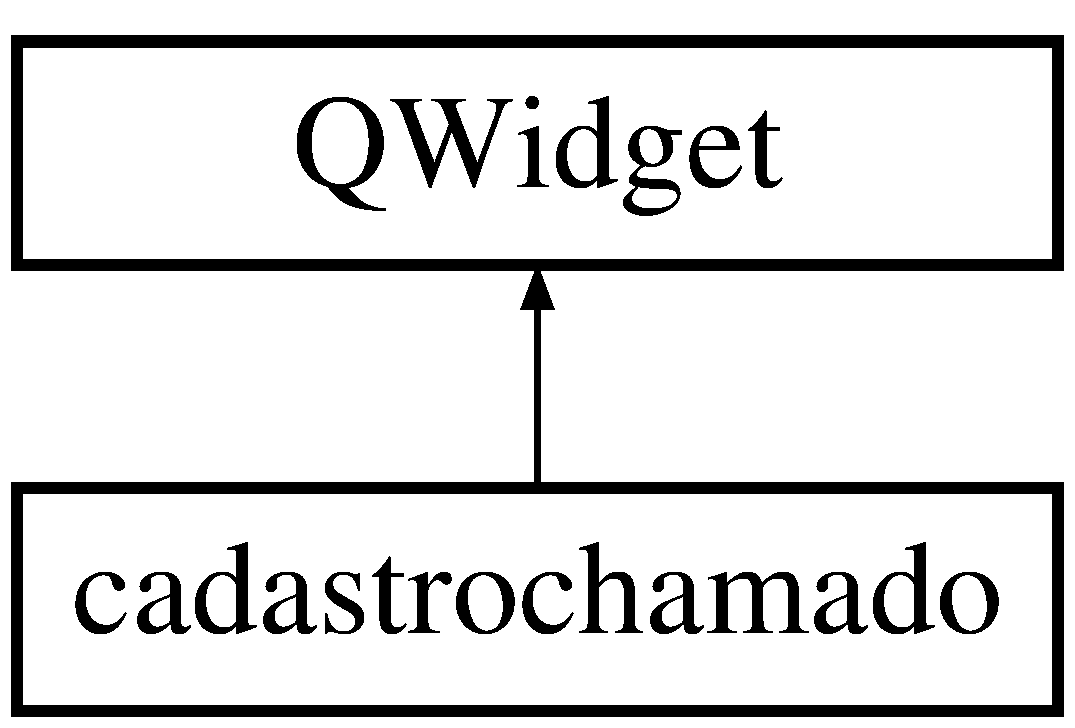
\includegraphics[height=2.000000cm]{classcadastrochamado}
\end{center}
\end{figure}
\subsection*{Public Member Functions}
\begin{DoxyCompactItemize}
\item 
{\bfseries cadastrochamado} (Q\+Widget $\ast$parent=0)\label{classcadastrochamado_a626bec1c5a76c3fe062f70f3fe857c3f}

\end{DoxyCompactItemize}


The documentation for this class was generated from the following files\+:\begin{DoxyCompactItemize}
\item 
D\+:/\+Users/\+Bruno/\+Documents/\+T\+C\+C\+\_\+\+Nay\+Bru/cadastrochamado.\+h\item 
D\+:/\+Users/\+Bruno/\+Documents/\+T\+C\+C\+\_\+\+Nay\+Bru/cadastrochamado.\+cpp\end{DoxyCompactItemize}

\hypertarget{classcadastrodispositivo}{}\section{cadastrodispositivo Class Reference}
\label{classcadastrodispositivo}\index{cadastrodispositivo@{cadastrodispositivo}}


{\ttfamily \#include $<$cadastrodispositivo.\+h$>$}

Inheritance diagram for cadastrodispositivo\+:\begin{figure}[H]
\begin{center}
\leavevmode
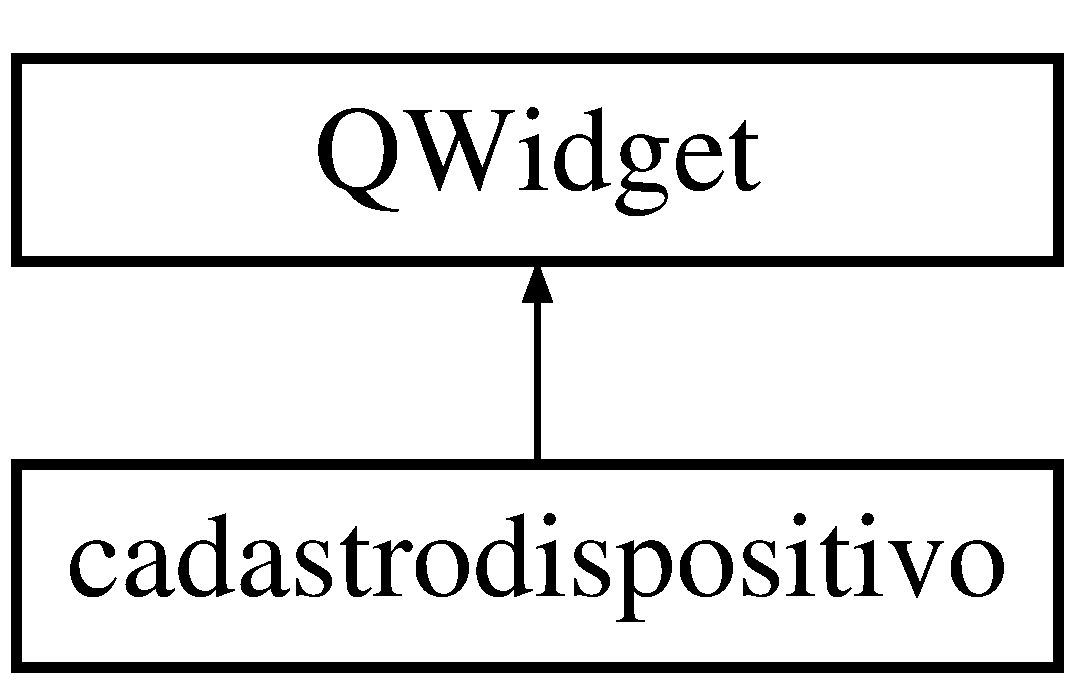
\includegraphics[height=2.000000cm]{classcadastrodispositivo}
\end{center}
\end{figure}
\subsection*{Public Member Functions}
\begin{DoxyCompactItemize}
\item 
\hyperlink{classcadastrodispositivo_a759ec481f21cb002c55d5ca50e8cdf9c}{cadastrodispositivo} (Q\+Widget $\ast$parent=0)
\item 
\hyperlink{classcadastrodispositivo_a21c4cb426f58445706d55dbce57f4aa0}{$\sim$cadastrodispositivo} ()
\end{DoxyCompactItemize}


\subsection{Detailed Description}


Definition at line 10 of file cadastrodispositivo.\+h.



\subsection{Constructor \& Destructor Documentation}
\hypertarget{classcadastrodispositivo_a759ec481f21cb002c55d5ca50e8cdf9c}{}\label{classcadastrodispositivo_a759ec481f21cb002c55d5ca50e8cdf9c} 
\index{cadastrodispositivo@{cadastrodispositivo}!cadastrodispositivo@{cadastrodispositivo}}
\index{cadastrodispositivo@{cadastrodispositivo}!cadastrodispositivo@{cadastrodispositivo}}
\subsubsection{\texorpdfstring{cadastrodispositivo()}{cadastrodispositivo()}}
{\footnotesize\ttfamily cadastrodispositivo\+::cadastrodispositivo (\begin{DoxyParamCaption}\item[{Q\+Widget $\ast$}]{parent = {\ttfamily 0} }\end{DoxyParamCaption})\hspace{0.3cm}{\ttfamily [explicit]}}



Definition at line 5 of file cadastrodispositivo.\+cpp.

\hypertarget{classcadastrodispositivo_a21c4cb426f58445706d55dbce57f4aa0}{}\label{classcadastrodispositivo_a21c4cb426f58445706d55dbce57f4aa0} 
\index{cadastrodispositivo@{cadastrodispositivo}!````~cadastrodispositivo@{$\sim$cadastrodispositivo}}
\index{````~cadastrodispositivo@{$\sim$cadastrodispositivo}!cadastrodispositivo@{cadastrodispositivo}}
\subsubsection{\texorpdfstring{$\sim$cadastrodispositivo()}{~cadastrodispositivo()}}
{\footnotesize\ttfamily cadastrodispositivo\+::$\sim$cadastrodispositivo (\begin{DoxyParamCaption}{ }\end{DoxyParamCaption})}



Definition at line 12 of file cadastrodispositivo.\+cpp.



The documentation for this class was generated from the following files\+:\begin{DoxyCompactItemize}
\item 
C\+:/\+Users/\+Bruno\+S\+R/\+T\+C\+C\+\_\+\+Nay\+Bru/\hyperlink{cadastrodispositivo_8h}{cadastrodispositivo.\+h}\item 
C\+:/\+Users/\+Bruno\+S\+R/\+T\+C\+C\+\_\+\+Nay\+Bru/\hyperlink{cadastrodispositivo_8cpp}{cadastrodispositivo.\+cpp}\end{DoxyCompactItemize}

\hypertarget{class_cadastropessoa}{}\section{Cadastropessoa Class Reference}
\label{class_cadastropessoa}\index{Cadastropessoa@{Cadastropessoa}}


{\ttfamily \#include $<$cadastropessoa.\+h$>$}

Inheritance diagram for Cadastropessoa\+:\begin{figure}[H]
\begin{center}
\leavevmode
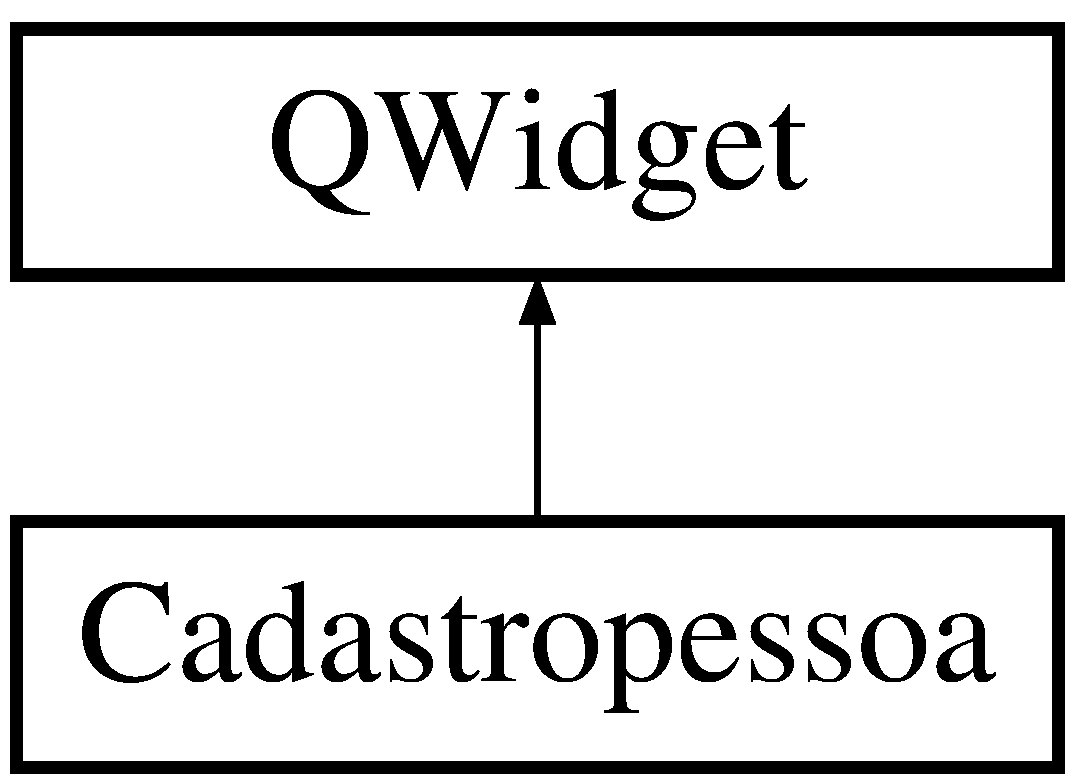
\includegraphics[height=2.000000cm]{class_cadastropessoa}
\end{center}
\end{figure}
\subsection*{Public Member Functions}
\begin{DoxyCompactItemize}
\item 
\hyperlink{class_cadastropessoa_a706230f399727160a6fd25592f77da12}{Cadastropessoa} (Q\+Widget $\ast$parent=0)
\item 
\hyperlink{class_cadastropessoa_a19e6b26d15f77eb6844e67b1246661cf}{$\sim$\+Cadastropessoa} ()
\end{DoxyCompactItemize}


\subsection{Detailed Description}


Definition at line 10 of file cadastropessoa.\+h.



\subsection{Constructor \& Destructor Documentation}
\hypertarget{class_cadastropessoa_a706230f399727160a6fd25592f77da12}{}\label{class_cadastropessoa_a706230f399727160a6fd25592f77da12} 
\index{Cadastropessoa@{Cadastropessoa}!Cadastropessoa@{Cadastropessoa}}
\index{Cadastropessoa@{Cadastropessoa}!Cadastropessoa@{Cadastropessoa}}
\subsubsection{\texorpdfstring{Cadastropessoa()}{Cadastropessoa()}}
{\footnotesize\ttfamily Cadastropessoa\+::\+Cadastropessoa (\begin{DoxyParamCaption}\item[{Q\+Widget $\ast$}]{parent = {\ttfamily 0} }\end{DoxyParamCaption})\hspace{0.3cm}{\ttfamily [explicit]}}



Definition at line 5 of file cadastropessoa.\+cpp.

\hypertarget{class_cadastropessoa_a19e6b26d15f77eb6844e67b1246661cf}{}\label{class_cadastropessoa_a19e6b26d15f77eb6844e67b1246661cf} 
\index{Cadastropessoa@{Cadastropessoa}!````~Cadastropessoa@{$\sim$\+Cadastropessoa}}
\index{````~Cadastropessoa@{$\sim$\+Cadastropessoa}!Cadastropessoa@{Cadastropessoa}}
\subsubsection{\texorpdfstring{$\sim$\+Cadastropessoa()}{~Cadastropessoa()}}
{\footnotesize\ttfamily Cadastropessoa\+::$\sim$\+Cadastropessoa (\begin{DoxyParamCaption}{ }\end{DoxyParamCaption})}



Definition at line 12 of file cadastropessoa.\+cpp.



The documentation for this class was generated from the following files\+:\begin{DoxyCompactItemize}
\item 
C\+:/\+Users/\+Bruno\+S\+R/\+T\+C\+C\+\_\+\+Nay\+Bru/\hyperlink{cadastropessoa_8h}{cadastropessoa.\+h}\item 
C\+:/\+Users/\+Bruno\+S\+R/\+T\+C\+C\+\_\+\+Nay\+Bru/\hyperlink{cadastropessoa_8cpp}{cadastropessoa.\+cpp}\end{DoxyCompactItemize}

\hypertarget{class_chamado}{}\section{Chamado Class Reference}
\label{class_chamado}\index{Chamado@{Chamado}}


{\ttfamily \#include $<$chamado.\+h$>$}

\subsection*{Public Member Functions}
\begin{DoxyCompactItemize}
\item 
\hyperlink{class_chamado_aeca5f123901cef6b33104291dc3b2fc0}{Chamado} ()
\item 
int \hyperlink{class_chamado_af8c3890123d55faf3a9adc2a274daaf2}{get\+Id} () const
\item 
void \hyperlink{class_chamado_ad9d1c6ef5c44c56921711fa96ae27277}{set\+Id} (int value)
\item 
\hyperlink{class_m_raci}{M\+Raci} \hyperlink{class_chamado_a99eef2190042baefb398806d35372edd}{get\+Matriz\+\_\+r} () const
\item 
void \hyperlink{class_chamado_a5f8f04ee1b58b3bbb46f8ba6a9c22342}{set\+Matriz\+\_\+r} (const \hyperlink{class_m_raci}{M\+Raci} \&value)
\item 
\hyperlink{class_dispositivo}{Dispositivo} \hyperlink{class_chamado_a1388c89d1f5ae80b7cfac8106c48dbc9}{get\+Disp} () const
\item 
void \hyperlink{class_chamado_aedfd2171f66178c80462e0477b49a0f0}{set\+Disp} (const \hyperlink{class_dispositivo}{Dispositivo} \&value)
\item 
float \hyperlink{class_chamado_abbe9ba6e55ea448b02e9c091369c1d2a}{get\+Tempo} () const
\item 
void \hyperlink{class_chamado_a918eb6053797974911821b777695b0c2}{set\+Tempo} (float value)
\item 
\hyperlink{class_status}{Status} \hyperlink{class_chamado_aa3f9a0756cd55a435fcbec3419a328dc}{get\+Stat} () const
\item 
void \hyperlink{class_chamado_a8a695ce190dcd9acf05e8b7880579fec}{set\+Stat} (const \hyperlink{class_status}{Status} \&value)
\item 
bool \hyperlink{class_chamado_ad481bcca8ee859304d67728bff772b10}{get\+Reincidente} () const
\item 
void \hyperlink{class_chamado_a0abb993bda04f1bd32ed474abf06d0ad}{set\+Reincidente} (bool value)
\item 
Q\+String \hyperlink{class_chamado_a58fd1c5cf9693ccc2ebacc9e7b984de0}{get\+Hora\+\_\+abertura} () const
\item 
void \hyperlink{class_chamado_a2513e3474003230bee760aeb28da8188}{set\+Hora\+\_\+abertura} (const Q\+String \&value)
\item 
Q\+String \hyperlink{class_chamado_a8d6f16bed156bb8241d1068ebe962483}{get\+Hora\+\_\+fechamento} () const
\item 
void \hyperlink{class_chamado_a4517fc2b385ef3ed227289c3444a0208}{set\+Hora\+\_\+fechamento} (const Q\+String \&value)
\item 
Q\+String \hyperlink{class_chamado_aa7aeb5e538449b9a71271756d7b39d43}{get\+Descricao} () const
\item 
void \hyperlink{class_chamado_a970a71741ec450c40c48eb4babd2fec3}{set\+Descricao} (const Q\+String \&value)
\end{DoxyCompactItemize}


\subsection{Detailed Description}


Definition at line 11 of file chamado.\+h.



\subsection{Constructor \& Destructor Documentation}
\hypertarget{class_chamado_aeca5f123901cef6b33104291dc3b2fc0}{}\label{class_chamado_aeca5f123901cef6b33104291dc3b2fc0} 
\index{Chamado@{Chamado}!Chamado@{Chamado}}
\index{Chamado@{Chamado}!Chamado@{Chamado}}
\subsubsection{\texorpdfstring{Chamado()}{Chamado()}}
{\footnotesize\ttfamily Chamado\+::\+Chamado (\begin{DoxyParamCaption}{ }\end{DoxyParamCaption})}



Definition at line 93 of file chamado.\+cpp.



\subsection{Member Function Documentation}
\hypertarget{class_chamado_aa7aeb5e538449b9a71271756d7b39d43}{}\label{class_chamado_aa7aeb5e538449b9a71271756d7b39d43} 
\index{Chamado@{Chamado}!get\+Descricao@{get\+Descricao}}
\index{get\+Descricao@{get\+Descricao}!Chamado@{Chamado}}
\subsubsection{\texorpdfstring{get\+Descricao()}{getDescricao()}}
{\footnotesize\ttfamily Q\+String Chamado\+::get\+Descricao (\begin{DoxyParamCaption}{ }\end{DoxyParamCaption}) const}



Definition at line 83 of file chamado.\+cpp.

\hypertarget{class_chamado_a1388c89d1f5ae80b7cfac8106c48dbc9}{}\label{class_chamado_a1388c89d1f5ae80b7cfac8106c48dbc9} 
\index{Chamado@{Chamado}!get\+Disp@{get\+Disp}}
\index{get\+Disp@{get\+Disp}!Chamado@{Chamado}}
\subsubsection{\texorpdfstring{get\+Disp()}{getDisp()}}
{\footnotesize\ttfamily \hyperlink{class_dispositivo}{Dispositivo} Chamado\+::get\+Disp (\begin{DoxyParamCaption}{ }\end{DoxyParamCaption}) const}



Definition at line 23 of file chamado.\+cpp.

\hypertarget{class_chamado_a58fd1c5cf9693ccc2ebacc9e7b984de0}{}\label{class_chamado_a58fd1c5cf9693ccc2ebacc9e7b984de0} 
\index{Chamado@{Chamado}!get\+Hora\+\_\+abertura@{get\+Hora\+\_\+abertura}}
\index{get\+Hora\+\_\+abertura@{get\+Hora\+\_\+abertura}!Chamado@{Chamado}}
\subsubsection{\texorpdfstring{get\+Hora\+\_\+abertura()}{getHora\_abertura()}}
{\footnotesize\ttfamily Q\+String Chamado\+::get\+Hora\+\_\+abertura (\begin{DoxyParamCaption}{ }\end{DoxyParamCaption}) const}



Definition at line 63 of file chamado.\+cpp.

\hypertarget{class_chamado_a8d6f16bed156bb8241d1068ebe962483}{}\label{class_chamado_a8d6f16bed156bb8241d1068ebe962483} 
\index{Chamado@{Chamado}!get\+Hora\+\_\+fechamento@{get\+Hora\+\_\+fechamento}}
\index{get\+Hora\+\_\+fechamento@{get\+Hora\+\_\+fechamento}!Chamado@{Chamado}}
\subsubsection{\texorpdfstring{get\+Hora\+\_\+fechamento()}{getHora\_fechamento()}}
{\footnotesize\ttfamily Q\+String Chamado\+::get\+Hora\+\_\+fechamento (\begin{DoxyParamCaption}{ }\end{DoxyParamCaption}) const}



Definition at line 73 of file chamado.\+cpp.

\hypertarget{class_chamado_af8c3890123d55faf3a9adc2a274daaf2}{}\label{class_chamado_af8c3890123d55faf3a9adc2a274daaf2} 
\index{Chamado@{Chamado}!get\+Id@{get\+Id}}
\index{get\+Id@{get\+Id}!Chamado@{Chamado}}
\subsubsection{\texorpdfstring{get\+Id()}{getId()}}
{\footnotesize\ttfamily int Chamado\+::get\+Id (\begin{DoxyParamCaption}{ }\end{DoxyParamCaption}) const}



Definition at line 3 of file chamado.\+cpp.

\hypertarget{class_chamado_a99eef2190042baefb398806d35372edd}{}\label{class_chamado_a99eef2190042baefb398806d35372edd} 
\index{Chamado@{Chamado}!get\+Matriz\+\_\+r@{get\+Matriz\+\_\+r}}
\index{get\+Matriz\+\_\+r@{get\+Matriz\+\_\+r}!Chamado@{Chamado}}
\subsubsection{\texorpdfstring{get\+Matriz\+\_\+r()}{getMatriz\_r()}}
{\footnotesize\ttfamily \hyperlink{class_m_raci}{M\+Raci} Chamado\+::get\+Matriz\+\_\+r (\begin{DoxyParamCaption}{ }\end{DoxyParamCaption}) const}



Definition at line 13 of file chamado.\+cpp.

\hypertarget{class_chamado_ad481bcca8ee859304d67728bff772b10}{}\label{class_chamado_ad481bcca8ee859304d67728bff772b10} 
\index{Chamado@{Chamado}!get\+Reincidente@{get\+Reincidente}}
\index{get\+Reincidente@{get\+Reincidente}!Chamado@{Chamado}}
\subsubsection{\texorpdfstring{get\+Reincidente()}{getReincidente()}}
{\footnotesize\ttfamily bool Chamado\+::get\+Reincidente (\begin{DoxyParamCaption}{ }\end{DoxyParamCaption}) const}



Definition at line 53 of file chamado.\+cpp.

\hypertarget{class_chamado_aa3f9a0756cd55a435fcbec3419a328dc}{}\label{class_chamado_aa3f9a0756cd55a435fcbec3419a328dc} 
\index{Chamado@{Chamado}!get\+Stat@{get\+Stat}}
\index{get\+Stat@{get\+Stat}!Chamado@{Chamado}}
\subsubsection{\texorpdfstring{get\+Stat()}{getStat()}}
{\footnotesize\ttfamily \hyperlink{class_status}{Status} Chamado\+::get\+Stat (\begin{DoxyParamCaption}{ }\end{DoxyParamCaption}) const}



Definition at line 43 of file chamado.\+cpp.

\hypertarget{class_chamado_abbe9ba6e55ea448b02e9c091369c1d2a}{}\label{class_chamado_abbe9ba6e55ea448b02e9c091369c1d2a} 
\index{Chamado@{Chamado}!get\+Tempo@{get\+Tempo}}
\index{get\+Tempo@{get\+Tempo}!Chamado@{Chamado}}
\subsubsection{\texorpdfstring{get\+Tempo()}{getTempo()}}
{\footnotesize\ttfamily float Chamado\+::get\+Tempo (\begin{DoxyParamCaption}{ }\end{DoxyParamCaption}) const}



Definition at line 33 of file chamado.\+cpp.

\hypertarget{class_chamado_a970a71741ec450c40c48eb4babd2fec3}{}\label{class_chamado_a970a71741ec450c40c48eb4babd2fec3} 
\index{Chamado@{Chamado}!set\+Descricao@{set\+Descricao}}
\index{set\+Descricao@{set\+Descricao}!Chamado@{Chamado}}
\subsubsection{\texorpdfstring{set\+Descricao()}{setDescricao()}}
{\footnotesize\ttfamily void Chamado\+::set\+Descricao (\begin{DoxyParamCaption}\item[{const Q\+String \&}]{value }\end{DoxyParamCaption})}



Definition at line 88 of file chamado.\+cpp.

\hypertarget{class_chamado_aedfd2171f66178c80462e0477b49a0f0}{}\label{class_chamado_aedfd2171f66178c80462e0477b49a0f0} 
\index{Chamado@{Chamado}!set\+Disp@{set\+Disp}}
\index{set\+Disp@{set\+Disp}!Chamado@{Chamado}}
\subsubsection{\texorpdfstring{set\+Disp()}{setDisp()}}
{\footnotesize\ttfamily void Chamado\+::set\+Disp (\begin{DoxyParamCaption}\item[{const \hyperlink{class_dispositivo}{Dispositivo} \&}]{value }\end{DoxyParamCaption})}



Definition at line 28 of file chamado.\+cpp.

\hypertarget{class_chamado_a2513e3474003230bee760aeb28da8188}{}\label{class_chamado_a2513e3474003230bee760aeb28da8188} 
\index{Chamado@{Chamado}!set\+Hora\+\_\+abertura@{set\+Hora\+\_\+abertura}}
\index{set\+Hora\+\_\+abertura@{set\+Hora\+\_\+abertura}!Chamado@{Chamado}}
\subsubsection{\texorpdfstring{set\+Hora\+\_\+abertura()}{setHora\_abertura()}}
{\footnotesize\ttfamily void Chamado\+::set\+Hora\+\_\+abertura (\begin{DoxyParamCaption}\item[{const Q\+String \&}]{value }\end{DoxyParamCaption})}



Definition at line 68 of file chamado.\+cpp.

\hypertarget{class_chamado_a4517fc2b385ef3ed227289c3444a0208}{}\label{class_chamado_a4517fc2b385ef3ed227289c3444a0208} 
\index{Chamado@{Chamado}!set\+Hora\+\_\+fechamento@{set\+Hora\+\_\+fechamento}}
\index{set\+Hora\+\_\+fechamento@{set\+Hora\+\_\+fechamento}!Chamado@{Chamado}}
\subsubsection{\texorpdfstring{set\+Hora\+\_\+fechamento()}{setHora\_fechamento()}}
{\footnotesize\ttfamily void Chamado\+::set\+Hora\+\_\+fechamento (\begin{DoxyParamCaption}\item[{const Q\+String \&}]{value }\end{DoxyParamCaption})}



Definition at line 78 of file chamado.\+cpp.

\hypertarget{class_chamado_ad9d1c6ef5c44c56921711fa96ae27277}{}\label{class_chamado_ad9d1c6ef5c44c56921711fa96ae27277} 
\index{Chamado@{Chamado}!set\+Id@{set\+Id}}
\index{set\+Id@{set\+Id}!Chamado@{Chamado}}
\subsubsection{\texorpdfstring{set\+Id()}{setId()}}
{\footnotesize\ttfamily void Chamado\+::set\+Id (\begin{DoxyParamCaption}\item[{int}]{value }\end{DoxyParamCaption})}



Definition at line 8 of file chamado.\+cpp.

\hypertarget{class_chamado_a5f8f04ee1b58b3bbb46f8ba6a9c22342}{}\label{class_chamado_a5f8f04ee1b58b3bbb46f8ba6a9c22342} 
\index{Chamado@{Chamado}!set\+Matriz\+\_\+r@{set\+Matriz\+\_\+r}}
\index{set\+Matriz\+\_\+r@{set\+Matriz\+\_\+r}!Chamado@{Chamado}}
\subsubsection{\texorpdfstring{set\+Matriz\+\_\+r()}{setMatriz\_r()}}
{\footnotesize\ttfamily void Chamado\+::set\+Matriz\+\_\+r (\begin{DoxyParamCaption}\item[{const \hyperlink{class_m_raci}{M\+Raci} \&}]{value }\end{DoxyParamCaption})}



Definition at line 18 of file chamado.\+cpp.

\hypertarget{class_chamado_a0abb993bda04f1bd32ed474abf06d0ad}{}\label{class_chamado_a0abb993bda04f1bd32ed474abf06d0ad} 
\index{Chamado@{Chamado}!set\+Reincidente@{set\+Reincidente}}
\index{set\+Reincidente@{set\+Reincidente}!Chamado@{Chamado}}
\subsubsection{\texorpdfstring{set\+Reincidente()}{setReincidente()}}
{\footnotesize\ttfamily void Chamado\+::set\+Reincidente (\begin{DoxyParamCaption}\item[{bool}]{value }\end{DoxyParamCaption})}



Definition at line 58 of file chamado.\+cpp.

\hypertarget{class_chamado_a8a695ce190dcd9acf05e8b7880579fec}{}\label{class_chamado_a8a695ce190dcd9acf05e8b7880579fec} 
\index{Chamado@{Chamado}!set\+Stat@{set\+Stat}}
\index{set\+Stat@{set\+Stat}!Chamado@{Chamado}}
\subsubsection{\texorpdfstring{set\+Stat()}{setStat()}}
{\footnotesize\ttfamily void Chamado\+::set\+Stat (\begin{DoxyParamCaption}\item[{const \hyperlink{class_status}{Status} \&}]{value }\end{DoxyParamCaption})}



Definition at line 48 of file chamado.\+cpp.

\hypertarget{class_chamado_a918eb6053797974911821b777695b0c2}{}\label{class_chamado_a918eb6053797974911821b777695b0c2} 
\index{Chamado@{Chamado}!set\+Tempo@{set\+Tempo}}
\index{set\+Tempo@{set\+Tempo}!Chamado@{Chamado}}
\subsubsection{\texorpdfstring{set\+Tempo()}{setTempo()}}
{\footnotesize\ttfamily void Chamado\+::set\+Tempo (\begin{DoxyParamCaption}\item[{float}]{value }\end{DoxyParamCaption})}



Definition at line 38 of file chamado.\+cpp.



The documentation for this class was generated from the following files\+:\begin{DoxyCompactItemize}
\item 
C\+:/\+Users/\+Bruno\+S\+R/\+T\+C\+C\+\_\+\+Nay\+Bru/\hyperlink{chamado_8h}{chamado.\+h}\item 
C\+:/\+Users/\+Bruno\+S\+R/\+T\+C\+C\+\_\+\+Nay\+Bru/\hyperlink{chamado_8cpp}{chamado.\+cpp}\end{DoxyCompactItemize}

\hypertarget{class_dispositivo}{}\section{Dispositivo Class Reference}
\label{class_dispositivo}\index{Dispositivo@{Dispositivo}}


{\ttfamily \#include $<$dispositivo.\+h$>$}

\subsection*{Public Member Functions}
\begin{DoxyCompactItemize}
\item 
\hyperlink{class_dispositivo_a08b3611c10447a1519d7ebb72f47e30d}{Dispositivo} ()
\item 
int \hyperlink{class_dispositivo_a4d470c1481fd167db94e6be4f08a259c}{get\+Id} () const
\item 
void \hyperlink{class_dispositivo_a186a8fdf627e6e9326a196fa7ad59846}{set\+Id} (int value)
\item 
Q\+String \hyperlink{class_dispositivo_a463552b0487176c52c477d7951287b4b}{get\+Nome} () const
\item 
void \hyperlink{class_dispositivo_a8bafe761c02216dd6bc7465eb4ff0064}{set\+Nome} (const Q\+String \&value)
\item 
Q\+String \hyperlink{class_dispositivo_a29327cf38f2c0b021e1197f12d02bf9c}{get\+Local} () const
\item 
void \hyperlink{class_dispositivo_a033c98bd8e7be483677b06ead506fe9d}{set\+Local} (const Q\+String \&value)
\item 
\hyperlink{classtipod}{tipod} \hyperlink{class_dispositivo_a0242efd1a66cffb9e979432e941d68ca}{get\+Tipo} () const
\item 
void \hyperlink{class_dispositivo_ada239ce7b043c5ae4d426cf4f1d0cf8f}{set\+Tipo} (const \hyperlink{classtipod}{tipod} \&value)
\end{DoxyCompactItemize}


\subsection{Detailed Description}


Definition at line 11 of file dispositivo.\+h.



\subsection{Constructor \& Destructor Documentation}
\hypertarget{class_dispositivo_a08b3611c10447a1519d7ebb72f47e30d}{}\label{class_dispositivo_a08b3611c10447a1519d7ebb72f47e30d} 
\index{Dispositivo@{Dispositivo}!Dispositivo@{Dispositivo}}
\index{Dispositivo@{Dispositivo}!Dispositivo@{Dispositivo}}
\subsubsection{\texorpdfstring{Dispositivo()}{Dispositivo()}}
{\footnotesize\ttfamily Dispositivo\+::\+Dispositivo (\begin{DoxyParamCaption}{ }\end{DoxyParamCaption})}



Definition at line 43 of file dispositivo.\+cpp.



\subsection{Member Function Documentation}
\hypertarget{class_dispositivo_a4d470c1481fd167db94e6be4f08a259c}{}\label{class_dispositivo_a4d470c1481fd167db94e6be4f08a259c} 
\index{Dispositivo@{Dispositivo}!get\+Id@{get\+Id}}
\index{get\+Id@{get\+Id}!Dispositivo@{Dispositivo}}
\subsubsection{\texorpdfstring{get\+Id()}{getId()}}
{\footnotesize\ttfamily int Dispositivo\+::get\+Id (\begin{DoxyParamCaption}{ }\end{DoxyParamCaption}) const}



Definition at line 3 of file dispositivo.\+cpp.

\hypertarget{class_dispositivo_a29327cf38f2c0b021e1197f12d02bf9c}{}\label{class_dispositivo_a29327cf38f2c0b021e1197f12d02bf9c} 
\index{Dispositivo@{Dispositivo}!get\+Local@{get\+Local}}
\index{get\+Local@{get\+Local}!Dispositivo@{Dispositivo}}
\subsubsection{\texorpdfstring{get\+Local()}{getLocal()}}
{\footnotesize\ttfamily Q\+String Dispositivo\+::get\+Local (\begin{DoxyParamCaption}{ }\end{DoxyParamCaption}) const}



Definition at line 23 of file dispositivo.\+cpp.

\hypertarget{class_dispositivo_a463552b0487176c52c477d7951287b4b}{}\label{class_dispositivo_a463552b0487176c52c477d7951287b4b} 
\index{Dispositivo@{Dispositivo}!get\+Nome@{get\+Nome}}
\index{get\+Nome@{get\+Nome}!Dispositivo@{Dispositivo}}
\subsubsection{\texorpdfstring{get\+Nome()}{getNome()}}
{\footnotesize\ttfamily Q\+String Dispositivo\+::get\+Nome (\begin{DoxyParamCaption}{ }\end{DoxyParamCaption}) const}



Definition at line 13 of file dispositivo.\+cpp.

\hypertarget{class_dispositivo_a0242efd1a66cffb9e979432e941d68ca}{}\label{class_dispositivo_a0242efd1a66cffb9e979432e941d68ca} 
\index{Dispositivo@{Dispositivo}!get\+Tipo@{get\+Tipo}}
\index{get\+Tipo@{get\+Tipo}!Dispositivo@{Dispositivo}}
\subsubsection{\texorpdfstring{get\+Tipo()}{getTipo()}}
{\footnotesize\ttfamily \hyperlink{classtipod}{tipod} Dispositivo\+::get\+Tipo (\begin{DoxyParamCaption}{ }\end{DoxyParamCaption}) const}



Definition at line 33 of file dispositivo.\+cpp.

\hypertarget{class_dispositivo_a186a8fdf627e6e9326a196fa7ad59846}{}\label{class_dispositivo_a186a8fdf627e6e9326a196fa7ad59846} 
\index{Dispositivo@{Dispositivo}!set\+Id@{set\+Id}}
\index{set\+Id@{set\+Id}!Dispositivo@{Dispositivo}}
\subsubsection{\texorpdfstring{set\+Id()}{setId()}}
{\footnotesize\ttfamily void Dispositivo\+::set\+Id (\begin{DoxyParamCaption}\item[{int}]{value }\end{DoxyParamCaption})}



Definition at line 8 of file dispositivo.\+cpp.

\hypertarget{class_dispositivo_a033c98bd8e7be483677b06ead506fe9d}{}\label{class_dispositivo_a033c98bd8e7be483677b06ead506fe9d} 
\index{Dispositivo@{Dispositivo}!set\+Local@{set\+Local}}
\index{set\+Local@{set\+Local}!Dispositivo@{Dispositivo}}
\subsubsection{\texorpdfstring{set\+Local()}{setLocal()}}
{\footnotesize\ttfamily void Dispositivo\+::set\+Local (\begin{DoxyParamCaption}\item[{const Q\+String \&}]{value }\end{DoxyParamCaption})}



Definition at line 28 of file dispositivo.\+cpp.

\hypertarget{class_dispositivo_a8bafe761c02216dd6bc7465eb4ff0064}{}\label{class_dispositivo_a8bafe761c02216dd6bc7465eb4ff0064} 
\index{Dispositivo@{Dispositivo}!set\+Nome@{set\+Nome}}
\index{set\+Nome@{set\+Nome}!Dispositivo@{Dispositivo}}
\subsubsection{\texorpdfstring{set\+Nome()}{setNome()}}
{\footnotesize\ttfamily void Dispositivo\+::set\+Nome (\begin{DoxyParamCaption}\item[{const Q\+String \&}]{value }\end{DoxyParamCaption})}



Definition at line 18 of file dispositivo.\+cpp.

\hypertarget{class_dispositivo_ada239ce7b043c5ae4d426cf4f1d0cf8f}{}\label{class_dispositivo_ada239ce7b043c5ae4d426cf4f1d0cf8f} 
\index{Dispositivo@{Dispositivo}!set\+Tipo@{set\+Tipo}}
\index{set\+Tipo@{set\+Tipo}!Dispositivo@{Dispositivo}}
\subsubsection{\texorpdfstring{set\+Tipo()}{setTipo()}}
{\footnotesize\ttfamily void Dispositivo\+::set\+Tipo (\begin{DoxyParamCaption}\item[{const \hyperlink{classtipod}{tipod} \&}]{value }\end{DoxyParamCaption})}



Definition at line 38 of file dispositivo.\+cpp.



The documentation for this class was generated from the following files\+:\begin{DoxyCompactItemize}
\item 
C\+:/\+Users/\+Bruno\+S\+R/\+T\+C\+C\+\_\+\+Nay\+Bru/\hyperlink{dispositivo_8h}{dispositivo.\+h}\item 
C\+:/\+Users/\+Bruno\+S\+R/\+T\+C\+C\+\_\+\+Nay\+Bru/\hyperlink{dispositivo_8cpp}{dispositivo.\+cpp}\end{DoxyCompactItemize}

\hypertarget{classgerencia_chamados}{}\section{gerencia\+Chamados Class Reference}
\label{classgerencia_chamados}\index{gerencia\+Chamados@{gerencia\+Chamados}}


{\ttfamily \#include $<$gerenciachamados.\+h$>$}

Inheritance diagram for gerencia\+Chamados\+:\begin{figure}[H]
\begin{center}
\leavevmode
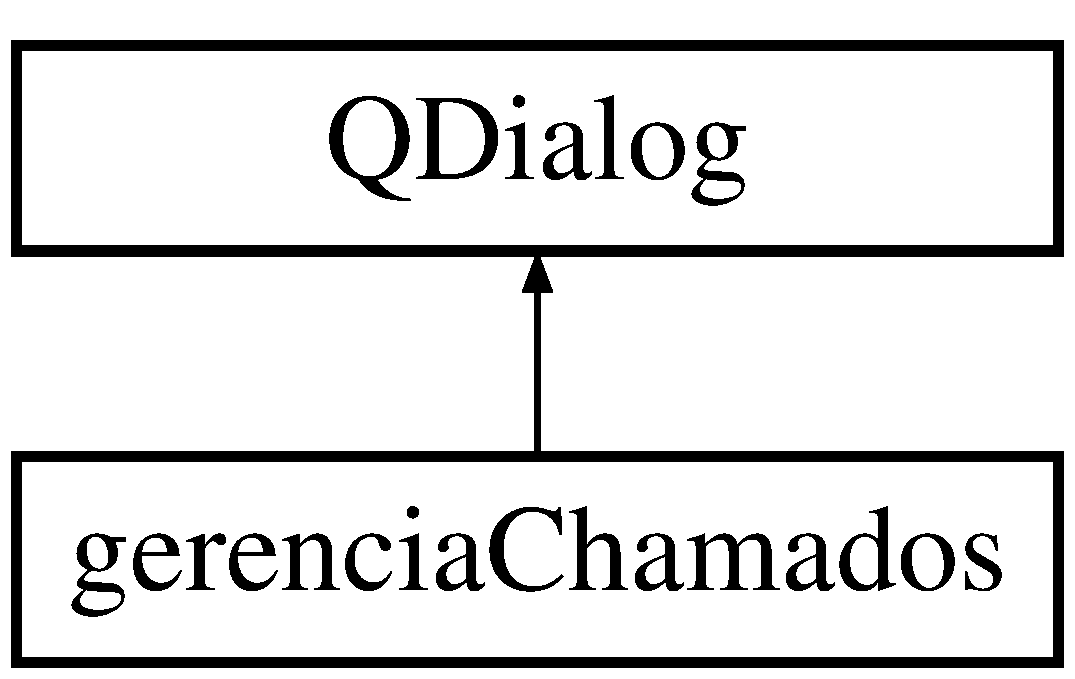
\includegraphics[height=2.000000cm]{classgerencia_chamados}
\end{center}
\end{figure}
\subsection*{Public Member Functions}
\begin{DoxyCompactItemize}
\item 
\hyperlink{classgerencia_chamados_a07839f849e9582ce8e695de48b4b0ebb}{gerencia\+Chamados} (Q\+Widget $\ast$parent=0)
\item 
\hyperlink{classgerencia_chamados_a393bdaec21bc5e91a03c4d4b02925682}{$\sim$gerencia\+Chamados} ()
\end{DoxyCompactItemize}


\subsection{Detailed Description}


Definition at line 10 of file gerenciachamados.\+h.



\subsection{Constructor \& Destructor Documentation}
\hypertarget{classgerencia_chamados_a07839f849e9582ce8e695de48b4b0ebb}{}\label{classgerencia_chamados_a07839f849e9582ce8e695de48b4b0ebb} 
\index{gerencia\+Chamados@{gerencia\+Chamados}!gerencia\+Chamados@{gerencia\+Chamados}}
\index{gerencia\+Chamados@{gerencia\+Chamados}!gerencia\+Chamados@{gerencia\+Chamados}}
\subsubsection{\texorpdfstring{gerencia\+Chamados()}{gerenciaChamados()}}
{\footnotesize\ttfamily gerencia\+Chamados\+::gerencia\+Chamados (\begin{DoxyParamCaption}\item[{Q\+Widget $\ast$}]{parent = {\ttfamily 0} }\end{DoxyParamCaption})\hspace{0.3cm}{\ttfamily [explicit]}}



Definition at line 5 of file gerenciachamados.\+cpp.

\hypertarget{classgerencia_chamados_a393bdaec21bc5e91a03c4d4b02925682}{}\label{classgerencia_chamados_a393bdaec21bc5e91a03c4d4b02925682} 
\index{gerencia\+Chamados@{gerencia\+Chamados}!````~gerencia\+Chamados@{$\sim$gerencia\+Chamados}}
\index{````~gerencia\+Chamados@{$\sim$gerencia\+Chamados}!gerencia\+Chamados@{gerencia\+Chamados}}
\subsubsection{\texorpdfstring{$\sim$gerencia\+Chamados()}{~gerenciaChamados()}}
{\footnotesize\ttfamily gerencia\+Chamados\+::$\sim$gerencia\+Chamados (\begin{DoxyParamCaption}{ }\end{DoxyParamCaption})}



Definition at line 12 of file gerenciachamados.\+cpp.



The documentation for this class was generated from the following files\+:\begin{DoxyCompactItemize}
\item 
C\+:/\+Users/\+Bruno\+S\+R/\+T\+C\+C\+\_\+\+Nay\+Bru/\hyperlink{gerenciachamados_8h}{gerenciachamados.\+h}\item 
C\+:/\+Users/\+Bruno\+S\+R/\+T\+C\+C\+\_\+\+Nay\+Bru/\hyperlink{gerenciachamados_8cpp}{gerenciachamados.\+cpp}\end{DoxyCompactItemize}

\hypertarget{classgerencia_dispositivo}{}\section{gerencia\+Dispositivo Class Reference}
\label{classgerencia_dispositivo}\index{gerencia\+Dispositivo@{gerencia\+Dispositivo}}


{\ttfamily \#include $<$gerenciadispositivo.\+h$>$}

Inheritance diagram for gerencia\+Dispositivo\+:\begin{figure}[H]
\begin{center}
\leavevmode
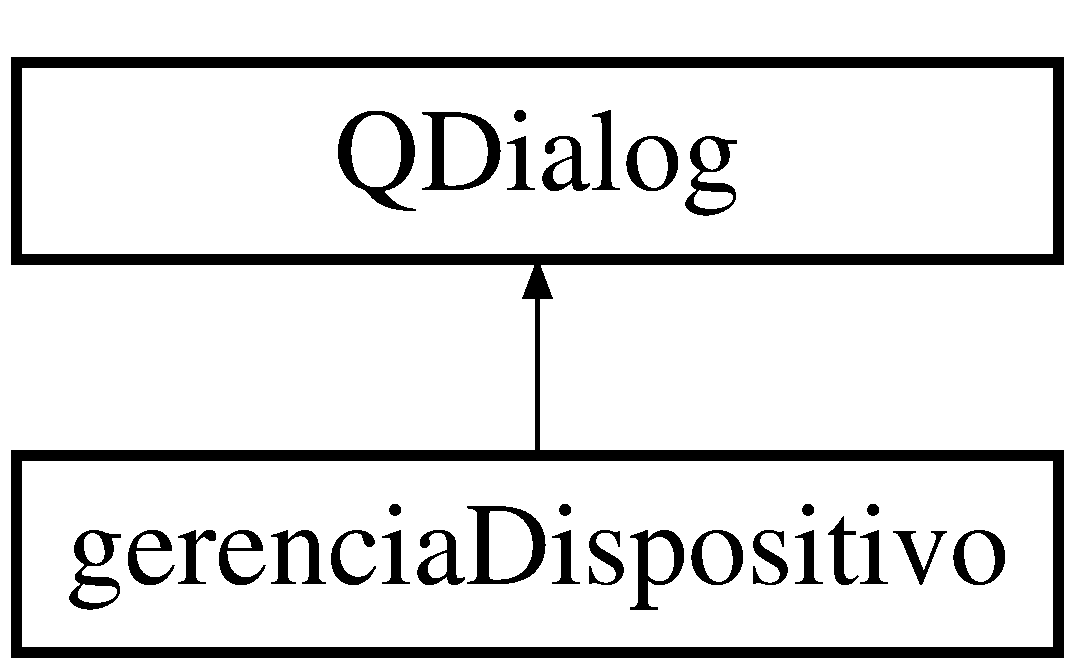
\includegraphics[height=2.000000cm]{classgerencia_dispositivo}
\end{center}
\end{figure}
\subsection*{Public Member Functions}
\begin{DoxyCompactItemize}
\item 
\hyperlink{classgerencia_dispositivo_a245e771cf0d5c9e2929e0829d57bf97b}{gerencia\+Dispositivo} (Q\+Widget $\ast$parent=0)
\item 
\hyperlink{classgerencia_dispositivo_a3dcef9c3f95ad6be653920a0952b8a0a}{$\sim$gerencia\+Dispositivo} ()
\end{DoxyCompactItemize}


\subsection{Detailed Description}


Definition at line 10 of file gerenciadispositivo.\+h.



\subsection{Constructor \& Destructor Documentation}
\hypertarget{classgerencia_dispositivo_a245e771cf0d5c9e2929e0829d57bf97b}{}\label{classgerencia_dispositivo_a245e771cf0d5c9e2929e0829d57bf97b} 
\index{gerencia\+Dispositivo@{gerencia\+Dispositivo}!gerencia\+Dispositivo@{gerencia\+Dispositivo}}
\index{gerencia\+Dispositivo@{gerencia\+Dispositivo}!gerencia\+Dispositivo@{gerencia\+Dispositivo}}
\subsubsection{\texorpdfstring{gerencia\+Dispositivo()}{gerenciaDispositivo()}}
{\footnotesize\ttfamily gerencia\+Dispositivo\+::gerencia\+Dispositivo (\begin{DoxyParamCaption}\item[{Q\+Widget $\ast$}]{parent = {\ttfamily 0} }\end{DoxyParamCaption})\hspace{0.3cm}{\ttfamily [explicit]}}



Definition at line 5 of file gerenciadispositivo.\+cpp.

\hypertarget{classgerencia_dispositivo_a3dcef9c3f95ad6be653920a0952b8a0a}{}\label{classgerencia_dispositivo_a3dcef9c3f95ad6be653920a0952b8a0a} 
\index{gerencia\+Dispositivo@{gerencia\+Dispositivo}!````~gerencia\+Dispositivo@{$\sim$gerencia\+Dispositivo}}
\index{````~gerencia\+Dispositivo@{$\sim$gerencia\+Dispositivo}!gerencia\+Dispositivo@{gerencia\+Dispositivo}}
\subsubsection{\texorpdfstring{$\sim$gerencia\+Dispositivo()}{~gerenciaDispositivo()}}
{\footnotesize\ttfamily gerencia\+Dispositivo\+::$\sim$gerencia\+Dispositivo (\begin{DoxyParamCaption}{ }\end{DoxyParamCaption})}



Definition at line 12 of file gerenciadispositivo.\+cpp.



The documentation for this class was generated from the following files\+:\begin{DoxyCompactItemize}
\item 
C\+:/\+Users/\+Bruno\+S\+R/\+T\+C\+C\+\_\+\+Nay\+Bru/\hyperlink{gerenciadispositivo_8h}{gerenciadispositivo.\+h}\item 
C\+:/\+Users/\+Bruno\+S\+R/\+T\+C\+C\+\_\+\+Nay\+Bru/\hyperlink{gerenciadispositivo_8cpp}{gerenciadispositivo.\+cpp}\end{DoxyCompactItemize}

\hypertarget{classgerencia_pessoas}{}\section{gerencia\+Pessoas Class Reference}
\label{classgerencia_pessoas}\index{gerencia\+Pessoas@{gerencia\+Pessoas}}


{\ttfamily \#include $<$gerenciapessoas.\+h$>$}

Inheritance diagram for gerencia\+Pessoas\+:\begin{figure}[H]
\begin{center}
\leavevmode
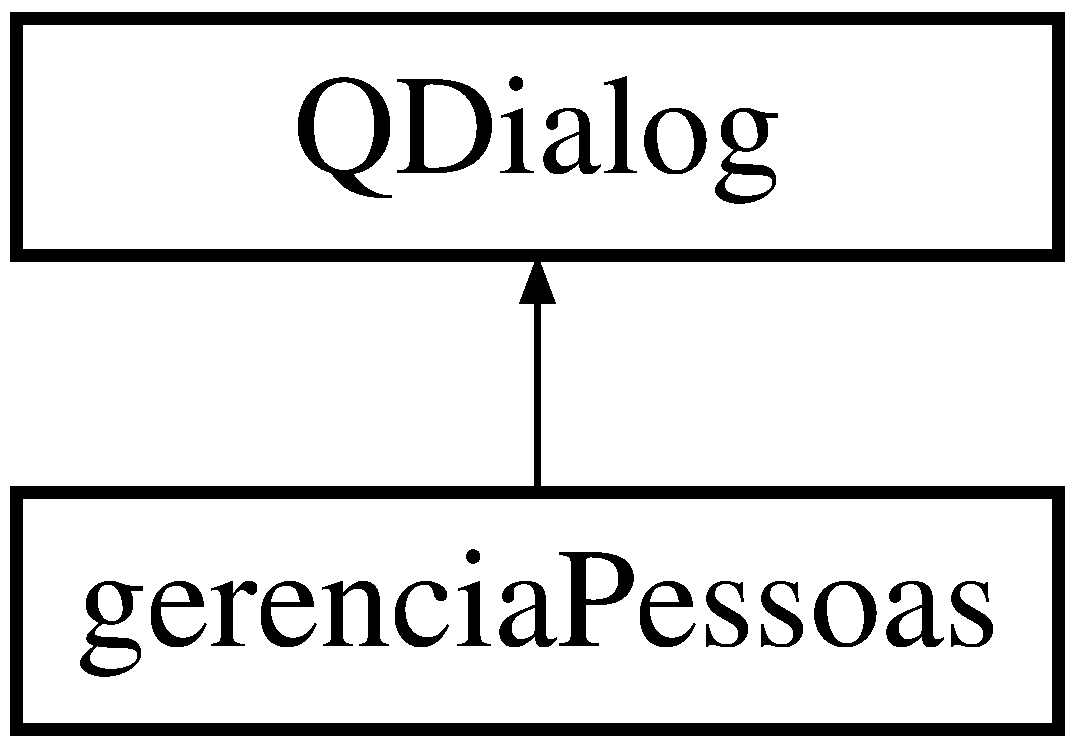
\includegraphics[height=2.000000cm]{classgerencia_pessoas}
\end{center}
\end{figure}
\subsection*{Public Member Functions}
\begin{DoxyCompactItemize}
\item 
\hyperlink{classgerencia_pessoas_a245ab3e4006fcdd3ec9a89815e1c60c1}{gerencia\+Pessoas} (Q\+Widget $\ast$parent=0)
\item 
\hyperlink{classgerencia_pessoas_a85f9272a309472903bf5b2ad0950973c}{$\sim$gerencia\+Pessoas} ()
\end{DoxyCompactItemize}


\subsection{Detailed Description}


Definition at line 10 of file gerenciapessoas.\+h.



\subsection{Constructor \& Destructor Documentation}
\hypertarget{classgerencia_pessoas_a245ab3e4006fcdd3ec9a89815e1c60c1}{}\label{classgerencia_pessoas_a245ab3e4006fcdd3ec9a89815e1c60c1} 
\index{gerencia\+Pessoas@{gerencia\+Pessoas}!gerencia\+Pessoas@{gerencia\+Pessoas}}
\index{gerencia\+Pessoas@{gerencia\+Pessoas}!gerencia\+Pessoas@{gerencia\+Pessoas}}
\subsubsection{\texorpdfstring{gerencia\+Pessoas()}{gerenciaPessoas()}}
{\footnotesize\ttfamily gerencia\+Pessoas\+::gerencia\+Pessoas (\begin{DoxyParamCaption}\item[{Q\+Widget $\ast$}]{parent = {\ttfamily 0} }\end{DoxyParamCaption})\hspace{0.3cm}{\ttfamily [explicit]}}



Definition at line 5 of file gerenciapessoas.\+cpp.

\hypertarget{classgerencia_pessoas_a85f9272a309472903bf5b2ad0950973c}{}\label{classgerencia_pessoas_a85f9272a309472903bf5b2ad0950973c} 
\index{gerencia\+Pessoas@{gerencia\+Pessoas}!````~gerencia\+Pessoas@{$\sim$gerencia\+Pessoas}}
\index{````~gerencia\+Pessoas@{$\sim$gerencia\+Pessoas}!gerencia\+Pessoas@{gerencia\+Pessoas}}
\subsubsection{\texorpdfstring{$\sim$gerencia\+Pessoas()}{~gerenciaPessoas()}}
{\footnotesize\ttfamily gerencia\+Pessoas\+::$\sim$gerencia\+Pessoas (\begin{DoxyParamCaption}{ }\end{DoxyParamCaption})}



Definition at line 12 of file gerenciapessoas.\+cpp.



The documentation for this class was generated from the following files\+:\begin{DoxyCompactItemize}
\item 
C\+:/\+Users/\+Bruno\+S\+R/\+T\+C\+C\+\_\+\+Nay\+Bru/\hyperlink{gerenciapessoas_8h}{gerenciapessoas.\+h}\item 
C\+:/\+Users/\+Bruno\+S\+R/\+T\+C\+C\+\_\+\+Nay\+Bru/\hyperlink{gerenciapessoas_8cpp}{gerenciapessoas.\+cpp}\end{DoxyCompactItemize}

\hypertarget{class_grupo_p}{}\section{GrupoP Class Reference}
\label{class_grupo_p}\index{GrupoP@{GrupoP}}


{\ttfamily \#include $<$grupop.\+h$>$}

\subsection*{Public Member Functions}
\begin{DoxyCompactItemize}
\item 
\hyperlink{class_grupo_p_aac812d0b4a0c443b7d7e36c00f60d23e}{GrupoP} ()
\item 
int \hyperlink{class_grupo_p_a3c72988138413046461c510b97ef7605}{get\+Id} () const
\item 
void \hyperlink{class_grupo_p_a540f8d78b7468b26b647485cc72fd7ca}{set\+Id} (int value)
\item 
Q\+String \hyperlink{class_grupo_p_ac3b0a8d64e082b45a7d362c69d934cd7}{get\+Nome} () const
\item 
void \hyperlink{class_grupo_p_af747750583e09cf0a1cfe756bacf97bc}{set\+Nome} (const Q\+String \&value)
\end{DoxyCompactItemize}


\subsection{Detailed Description}


Definition at line 5 of file grupop.\+h.



\subsection{Constructor \& Destructor Documentation}
\hypertarget{class_grupo_p_aac812d0b4a0c443b7d7e36c00f60d23e}{}\label{class_grupo_p_aac812d0b4a0c443b7d7e36c00f60d23e} 
\index{GrupoP@{GrupoP}!GrupoP@{GrupoP}}
\index{GrupoP@{GrupoP}!GrupoP@{GrupoP}}
\subsubsection{\texorpdfstring{Grupo\+P()}{GrupoP()}}
{\footnotesize\ttfamily Grupo\+P\+::\+GrupoP (\begin{DoxyParamCaption}{ }\end{DoxyParamCaption})}



Definition at line 23 of file grupop.\+cpp.



\subsection{Member Function Documentation}
\hypertarget{class_grupo_p_a3c72988138413046461c510b97ef7605}{}\label{class_grupo_p_a3c72988138413046461c510b97ef7605} 
\index{GrupoP@{GrupoP}!get\+Id@{get\+Id}}
\index{get\+Id@{get\+Id}!GrupoP@{GrupoP}}
\subsubsection{\texorpdfstring{get\+Id()}{getId()}}
{\footnotesize\ttfamily int Grupo\+P\+::get\+Id (\begin{DoxyParamCaption}{ }\end{DoxyParamCaption}) const}



Definition at line 3 of file grupop.\+cpp.

\hypertarget{class_grupo_p_ac3b0a8d64e082b45a7d362c69d934cd7}{}\label{class_grupo_p_ac3b0a8d64e082b45a7d362c69d934cd7} 
\index{GrupoP@{GrupoP}!get\+Nome@{get\+Nome}}
\index{get\+Nome@{get\+Nome}!GrupoP@{GrupoP}}
\subsubsection{\texorpdfstring{get\+Nome()}{getNome()}}
{\footnotesize\ttfamily Q\+String Grupo\+P\+::get\+Nome (\begin{DoxyParamCaption}{ }\end{DoxyParamCaption}) const}



Definition at line 13 of file grupop.\+cpp.

\hypertarget{class_grupo_p_a540f8d78b7468b26b647485cc72fd7ca}{}\label{class_grupo_p_a540f8d78b7468b26b647485cc72fd7ca} 
\index{GrupoP@{GrupoP}!set\+Id@{set\+Id}}
\index{set\+Id@{set\+Id}!GrupoP@{GrupoP}}
\subsubsection{\texorpdfstring{set\+Id()}{setId()}}
{\footnotesize\ttfamily void Grupo\+P\+::set\+Id (\begin{DoxyParamCaption}\item[{int}]{value }\end{DoxyParamCaption})}



Definition at line 8 of file grupop.\+cpp.

\hypertarget{class_grupo_p_af747750583e09cf0a1cfe756bacf97bc}{}\label{class_grupo_p_af747750583e09cf0a1cfe756bacf97bc} 
\index{GrupoP@{GrupoP}!set\+Nome@{set\+Nome}}
\index{set\+Nome@{set\+Nome}!GrupoP@{GrupoP}}
\subsubsection{\texorpdfstring{set\+Nome()}{setNome()}}
{\footnotesize\ttfamily void Grupo\+P\+::set\+Nome (\begin{DoxyParamCaption}\item[{const Q\+String \&}]{value }\end{DoxyParamCaption})}



Definition at line 18 of file grupop.\+cpp.



The documentation for this class was generated from the following files\+:\begin{DoxyCompactItemize}
\item 
C\+:/\+Users/\+Bruno\+S\+R/\+T\+C\+C\+\_\+\+Nay\+Bru/\hyperlink{grupop_8h}{grupop.\+h}\item 
C\+:/\+Users/\+Bruno\+S\+R/\+T\+C\+C\+\_\+\+Nay\+Bru/\hyperlink{grupop_8cpp}{grupop.\+cpp}\end{DoxyCompactItemize}

\hypertarget{class_main_window}{}\section{Main\+Window Class Reference}
\label{class_main_window}\index{Main\+Window@{Main\+Window}}


{\ttfamily \#include $<$mainwindow.\+h$>$}

Inheritance diagram for Main\+Window\+:\begin{figure}[H]
\begin{center}
\leavevmode
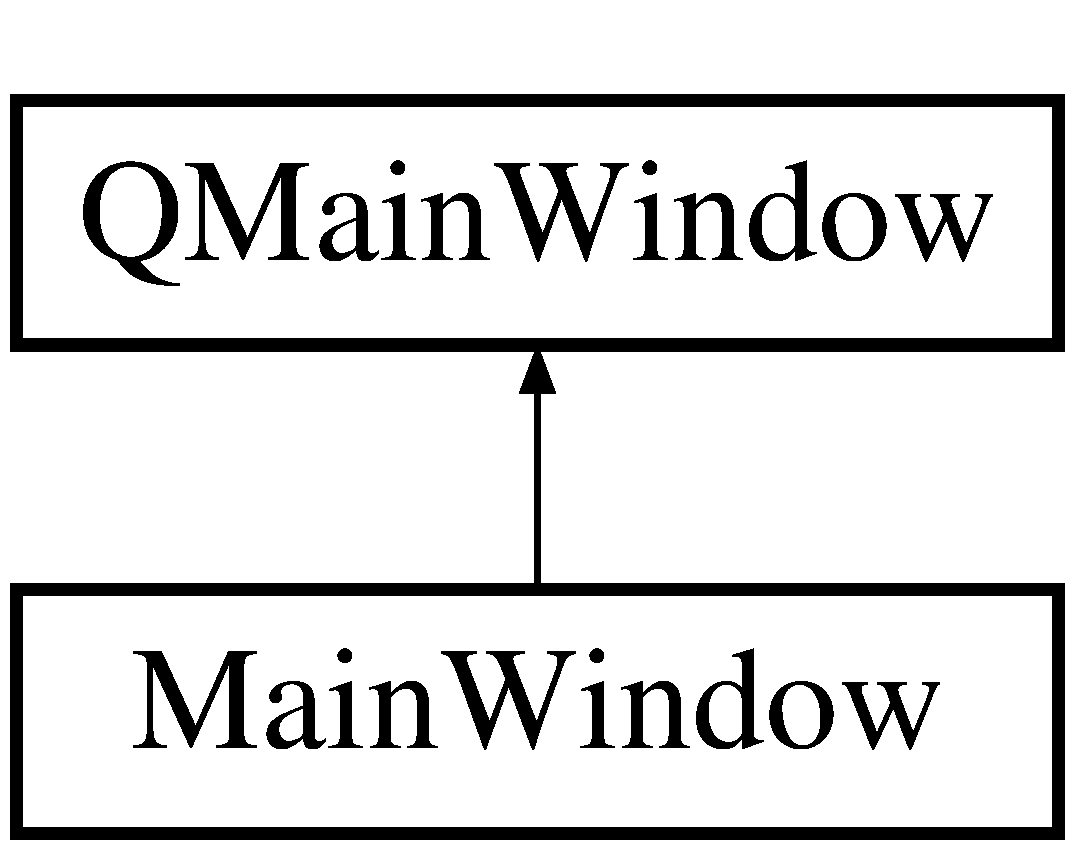
\includegraphics[height=2.000000cm]{class_main_window}
\end{center}
\end{figure}
\subsection*{Public Member Functions}
\begin{DoxyCompactItemize}
\item 
\hyperlink{class_main_window_a8b244be8b7b7db1b08de2a2acb9409db}{Main\+Window} (Q\+Widget $\ast$parent=0)
\item 
\hyperlink{class_main_window_ae98d00a93bc118200eeef9f9bba1dba7}{$\sim$\+Main\+Window} ()
\end{DoxyCompactItemize}


\subsection{Detailed Description}


Definition at line 27 of file mainwindow.\+h.



\subsection{Constructor \& Destructor Documentation}
\hypertarget{class_main_window_a8b244be8b7b7db1b08de2a2acb9409db}{}\label{class_main_window_a8b244be8b7b7db1b08de2a2acb9409db} 
\index{Main\+Window@{Main\+Window}!Main\+Window@{Main\+Window}}
\index{Main\+Window@{Main\+Window}!Main\+Window@{Main\+Window}}
\subsubsection{\texorpdfstring{Main\+Window()}{MainWindow()}}
{\footnotesize\ttfamily Main\+Window\+::\+Main\+Window (\begin{DoxyParamCaption}\item[{Q\+Widget $\ast$}]{parent = {\ttfamily 0} }\end{DoxyParamCaption})\hspace{0.3cm}{\ttfamily [explicit]}}



Definition at line 9 of file mainwindow.\+cpp.

\hypertarget{class_main_window_ae98d00a93bc118200eeef9f9bba1dba7}{}\label{class_main_window_ae98d00a93bc118200eeef9f9bba1dba7} 
\index{Main\+Window@{Main\+Window}!````~Main\+Window@{$\sim$\+Main\+Window}}
\index{````~Main\+Window@{$\sim$\+Main\+Window}!Main\+Window@{Main\+Window}}
\subsubsection{\texorpdfstring{$\sim$\+Main\+Window()}{~MainWindow()}}
{\footnotesize\ttfamily Main\+Window\+::$\sim$\+Main\+Window (\begin{DoxyParamCaption}{ }\end{DoxyParamCaption})}



Definition at line 17 of file mainwindow.\+cpp.



The documentation for this class was generated from the following files\+:\begin{DoxyCompactItemize}
\item 
C\+:/\+Users/\+Bruno\+S\+R/\+T\+C\+C\+\_\+\+Nay\+Bru/\hyperlink{mainwindow_8h}{mainwindow.\+h}\item 
C\+:/\+Users/\+Bruno\+S\+R/\+T\+C\+C\+\_\+\+Nay\+Bru/\hyperlink{mainwindow_8cpp}{mainwindow.\+cpp}\end{DoxyCompactItemize}

\section{matriz\+R\+A\+CI Class Reference}
\label{classmatriz_r_a_c_i}\index{matriz\+R\+A\+CI@{matriz\+R\+A\+CI}}
Inheritance diagram for matriz\+R\+A\+CI\+:\begin{figure}[H]
\begin{center}
\leavevmode
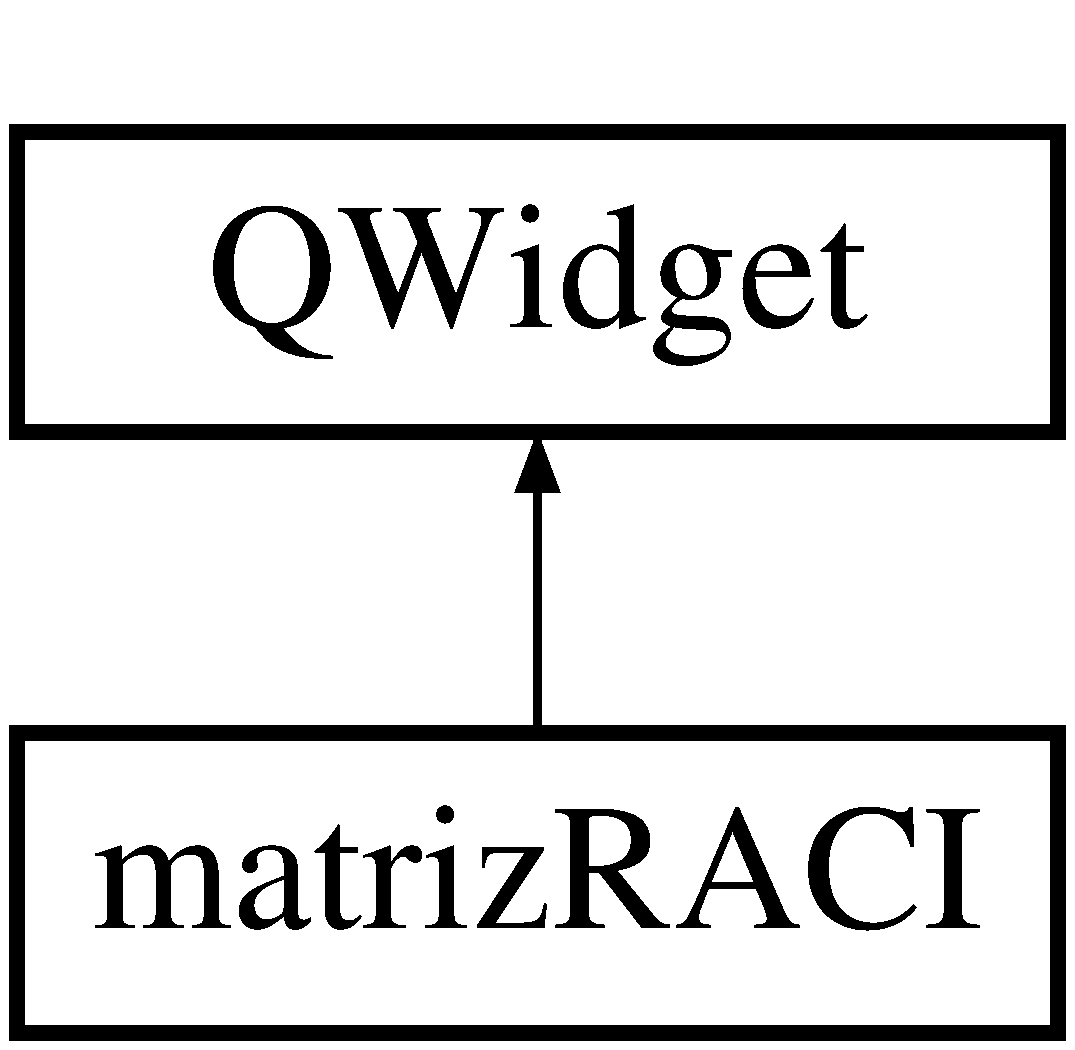
\includegraphics[height=2.000000cm]{classmatriz_r_a_c_i}
\end{center}
\end{figure}
\subsection*{Public Member Functions}
\begin{DoxyCompactItemize}
\item 
{\bfseries matriz\+R\+A\+CI} (Q\+Widget $\ast$parent=0)\label{classmatriz_r_a_c_i_ae380d9647713f9dc8c4dbc275f69a672}

\end{DoxyCompactItemize}


The documentation for this class was generated from the following files\+:\begin{DoxyCompactItemize}
\item 
D\+:/\+Users/\+Bruno/\+Documents/\+T\+C\+C\+\_\+\+Nay\+Bru/matrizraci.\+h\item 
D\+:/\+Users/\+Bruno/\+Documents/\+T\+C\+C\+\_\+\+Nay\+Bru/matrizraci.\+cpp\end{DoxyCompactItemize}

\hypertarget{class_m_raci}{}\section{M\+Raci Class Reference}
\label{class_m_raci}\index{M\+Raci@{M\+Raci}}


{\ttfamily \#include $<$m\+\_\+raci.\+h$>$}

\subsection*{Public Member Functions}
\begin{DoxyCompactItemize}
\item 
\hyperlink{class_m_raci_a62c738f5cf78b52066d235d7d159afe8}{M\+Raci} ()
\end{DoxyCompactItemize}


\subsection{Detailed Description}


Definition at line 8 of file m\+\_\+raci.\+h.



\subsection{Constructor \& Destructor Documentation}
\hypertarget{class_m_raci_a62c738f5cf78b52066d235d7d159afe8}{}\label{class_m_raci_a62c738f5cf78b52066d235d7d159afe8} 
\index{M\+Raci@{M\+Raci}!M\+Raci@{M\+Raci}}
\index{M\+Raci@{M\+Raci}!M\+Raci@{M\+Raci}}
\subsubsection{\texorpdfstring{M\+Raci()}{MRaci()}}
{\footnotesize\ttfamily M\+Raci\+::\+M\+Raci (\begin{DoxyParamCaption}{ }\end{DoxyParamCaption})}



Definition at line 5 of file m\+\_\+raci.\+cpp.



The documentation for this class was generated from the following files\+:\begin{DoxyCompactItemize}
\item 
C\+:/\+Users/\+Bruno\+S\+R/\+T\+C\+C\+\_\+\+Nay\+Bru/\hyperlink{m__raci_8h}{m\+\_\+raci.\+h}\item 
C\+:/\+Users/\+Bruno\+S\+R/\+T\+C\+C\+\_\+\+Nay\+Bru/\hyperlink{m__raci_8cpp}{m\+\_\+raci.\+cpp}\end{DoxyCompactItemize}

\hypertarget{classnovo_grupo}{}\section{novo\+Grupo Class Reference}
\label{classnovo_grupo}\index{novo\+Grupo@{novo\+Grupo}}


{\ttfamily \#include $<$novogrupo.\+h$>$}

Inheritance diagram for novo\+Grupo\+:\begin{figure}[H]
\begin{center}
\leavevmode
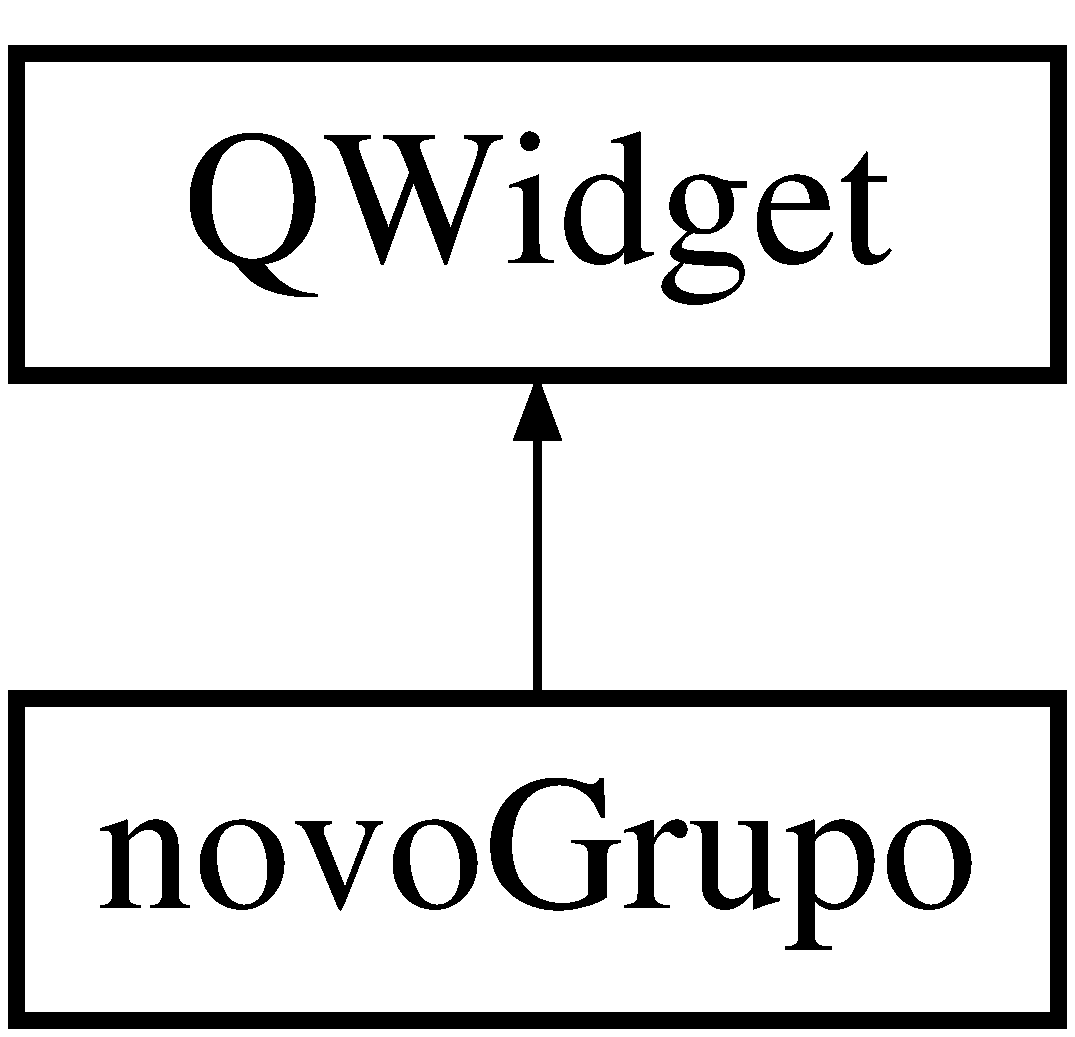
\includegraphics[height=2.000000cm]{classnovo_grupo}
\end{center}
\end{figure}
\subsection*{Public Member Functions}
\begin{DoxyCompactItemize}
\item 
\hyperlink{classnovo_grupo_a2e343a019db9fe74eea1809e833a8517}{novo\+Grupo} (Q\+Widget $\ast$parent=0)
\item 
\hyperlink{classnovo_grupo_a561957c27e43bc56cc595a37db18aa33}{$\sim$novo\+Grupo} ()
\end{DoxyCompactItemize}


\subsection{Detailed Description}


Definition at line 10 of file novogrupo.\+h.



\subsection{Constructor \& Destructor Documentation}
\hypertarget{classnovo_grupo_a2e343a019db9fe74eea1809e833a8517}{}\label{classnovo_grupo_a2e343a019db9fe74eea1809e833a8517} 
\index{novo\+Grupo@{novo\+Grupo}!novo\+Grupo@{novo\+Grupo}}
\index{novo\+Grupo@{novo\+Grupo}!novo\+Grupo@{novo\+Grupo}}
\subsubsection{\texorpdfstring{novo\+Grupo()}{novoGrupo()}}
{\footnotesize\ttfamily novo\+Grupo\+::novo\+Grupo (\begin{DoxyParamCaption}\item[{Q\+Widget $\ast$}]{parent = {\ttfamily 0} }\end{DoxyParamCaption})\hspace{0.3cm}{\ttfamily [explicit]}}



Definition at line 4 of file novogrupo.\+cpp.

\hypertarget{classnovo_grupo_a561957c27e43bc56cc595a37db18aa33}{}\label{classnovo_grupo_a561957c27e43bc56cc595a37db18aa33} 
\index{novo\+Grupo@{novo\+Grupo}!````~novo\+Grupo@{$\sim$novo\+Grupo}}
\index{````~novo\+Grupo@{$\sim$novo\+Grupo}!novo\+Grupo@{novo\+Grupo}}
\subsubsection{\texorpdfstring{$\sim$novo\+Grupo()}{~novoGrupo()}}
{\footnotesize\ttfamily novo\+Grupo\+::$\sim$novo\+Grupo (\begin{DoxyParamCaption}{ }\end{DoxyParamCaption})}



Definition at line 11 of file novogrupo.\+cpp.



The documentation for this class was generated from the following files\+:\begin{DoxyCompactItemize}
\item 
C\+:/\+Users/\+Bruno\+S\+R/\+T\+C\+C\+\_\+\+Nay\+Bru/\hyperlink{novogrupo_8h}{novogrupo.\+h}\item 
C\+:/\+Users/\+Bruno\+S\+R/\+T\+C\+C\+\_\+\+Nay\+Bru/\hyperlink{novogrupo_8cpp}{novogrupo.\+cpp}\end{DoxyCompactItemize}

\hypertarget{classpessoa}{}\section{pessoa Class Reference}
\label{classpessoa}\index{pessoa@{pessoa}}


{\ttfamily \#include $<$pessoa.\+h$>$}

\subsection*{Public Member Functions}
\begin{DoxyCompactItemize}
\item 
\hyperlink{classpessoa_ae2ee70812ff092a18c24ed94eaae260b}{pessoa} ()
\item 
int \hyperlink{classpessoa_a9a20cb67d382a667ad8ed10761b50211}{get\+Id} () const
\item 
void \hyperlink{classpessoa_ab528a41c403719b847f8e43c0893e14c}{set\+Id} (int value)
\item 
string \hyperlink{classpessoa_ad673a812f80d63efaef99aa84096ceb1}{get\+Nome} () const
\item 
void \hyperlink{classpessoa_a5e7a713ac30be9101a9d3d59848269e1}{set\+Nome} (const string \&value)
\item 
string \hyperlink{classpessoa_a248cbdf67320b616ba15c323dea16bb5}{get\+Telefone} () const
\item 
void \hyperlink{classpessoa_ae407991762018bfd08cf3f3d52262071}{set\+Telefone} (const string \&value)
\item 
int \hyperlink{classpessoa_afe3f63c712664c2ac32f89ed8595d75d}{get\+Ramal} () const
\item 
void \hyperlink{classpessoa_a4e6fa1b22e8824e270fd2aee4c9866e7}{set\+Ramal} (int value)
\item 
string \hyperlink{classpessoa_a41fc2c5db3716b88356b23987fd14bb4}{get\+Email} () const
\item 
void \hyperlink{classpessoa_ab5f43c9f7ab0b72df2758d4d1da92a63}{set\+Email} (const string \&value)
\item 
string \hyperlink{classpessoa_a7e0858513abeb0579b987e7a7a79f0d7}{get\+Depto} () const
\item 
void \hyperlink{classpessoa_ae71cc4caf660b5ffc4f9bedc5b4d9d79}{set\+Depto} (const string \&value)
\item 
string \hyperlink{classpessoa_aa4b0643f31c9d0e338ca7a485bc0723d}{get\+Cargo} () const
\item 
void \hyperlink{classpessoa_a9fd52a51b1f987c28aa8016899beb892}{set\+Cargo} (const string \&value)
\item 
int \hyperlink{classpessoa_ad1bad474adbfadf472ad857a7c5f181c}{get\+Grupo} () const
\item 
void \hyperlink{classpessoa_abde4772449869bd2c8e5e6d280e4f9f5}{set\+Grupo} (int value)
\end{DoxyCompactItemize}
\subsection*{Public Attributes}
\begin{DoxyCompactItemize}
\item 
int \hyperlink{classpessoa_a8e80bd7d70d7d29b248ef5ec77720b5b}{id}
\item 
string \hyperlink{classpessoa_a7ff09497b62adeb87afd1531d72dee78}{nome}
\item 
string \hyperlink{classpessoa_aa73d0148299c1920e2ab238956a869ab}{telefone}
\item 
int \hyperlink{classpessoa_a3263ed9356bab20fb6c364483fe0d7b7}{ramal}
\item 
string \hyperlink{classpessoa_a8629e223b05473916ecda357a5fe1ad1}{email}
\item 
string \hyperlink{classpessoa_ac75b9d5e9934fdcb46c0d8b2c06a08b2}{depto}
\item 
string \hyperlink{classpessoa_a32474b998586278afec16302178c2856}{cargo}
\item 
int \hyperlink{classpessoa_a6930db502e29734eb026e291cf534ed9}{grupo}
\end{DoxyCompactItemize}


\subsection{Detailed Description}


Definition at line 8 of file pessoa.\+h.



\subsection{Constructor \& Destructor Documentation}
\hypertarget{classpessoa_ae2ee70812ff092a18c24ed94eaae260b}{}\label{classpessoa_ae2ee70812ff092a18c24ed94eaae260b} 
\index{pessoa@{pessoa}!pessoa@{pessoa}}
\index{pessoa@{pessoa}!pessoa@{pessoa}}
\subsubsection{\texorpdfstring{pessoa()}{pessoa()}}
{\footnotesize\ttfamily pessoa\+::pessoa (\begin{DoxyParamCaption}{ }\end{DoxyParamCaption})}



Definition at line 83 of file pessoa.\+cpp.



\subsection{Member Function Documentation}
\hypertarget{classpessoa_aa4b0643f31c9d0e338ca7a485bc0723d}{}\label{classpessoa_aa4b0643f31c9d0e338ca7a485bc0723d} 
\index{pessoa@{pessoa}!get\+Cargo@{get\+Cargo}}
\index{get\+Cargo@{get\+Cargo}!pessoa@{pessoa}}
\subsubsection{\texorpdfstring{get\+Cargo()}{getCargo()}}
{\footnotesize\ttfamily string pessoa\+::get\+Cargo (\begin{DoxyParamCaption}{ }\end{DoxyParamCaption}) const}



Definition at line 63 of file pessoa.\+cpp.

\hypertarget{classpessoa_a7e0858513abeb0579b987e7a7a79f0d7}{}\label{classpessoa_a7e0858513abeb0579b987e7a7a79f0d7} 
\index{pessoa@{pessoa}!get\+Depto@{get\+Depto}}
\index{get\+Depto@{get\+Depto}!pessoa@{pessoa}}
\subsubsection{\texorpdfstring{get\+Depto()}{getDepto()}}
{\footnotesize\ttfamily string pessoa\+::get\+Depto (\begin{DoxyParamCaption}{ }\end{DoxyParamCaption}) const}



Definition at line 53 of file pessoa.\+cpp.

\hypertarget{classpessoa_a41fc2c5db3716b88356b23987fd14bb4}{}\label{classpessoa_a41fc2c5db3716b88356b23987fd14bb4} 
\index{pessoa@{pessoa}!get\+Email@{get\+Email}}
\index{get\+Email@{get\+Email}!pessoa@{pessoa}}
\subsubsection{\texorpdfstring{get\+Email()}{getEmail()}}
{\footnotesize\ttfamily string pessoa\+::get\+Email (\begin{DoxyParamCaption}{ }\end{DoxyParamCaption}) const}



Definition at line 43 of file pessoa.\+cpp.

\hypertarget{classpessoa_ad1bad474adbfadf472ad857a7c5f181c}{}\label{classpessoa_ad1bad474adbfadf472ad857a7c5f181c} 
\index{pessoa@{pessoa}!get\+Grupo@{get\+Grupo}}
\index{get\+Grupo@{get\+Grupo}!pessoa@{pessoa}}
\subsubsection{\texorpdfstring{get\+Grupo()}{getGrupo()}}
{\footnotesize\ttfamily int pessoa\+::get\+Grupo (\begin{DoxyParamCaption}{ }\end{DoxyParamCaption}) const}



Definition at line 73 of file pessoa.\+cpp.

\hypertarget{classpessoa_a9a20cb67d382a667ad8ed10761b50211}{}\label{classpessoa_a9a20cb67d382a667ad8ed10761b50211} 
\index{pessoa@{pessoa}!get\+Id@{get\+Id}}
\index{get\+Id@{get\+Id}!pessoa@{pessoa}}
\subsubsection{\texorpdfstring{get\+Id()}{getId()}}
{\footnotesize\ttfamily int pessoa\+::get\+Id (\begin{DoxyParamCaption}{ }\end{DoxyParamCaption}) const}



Definition at line 3 of file pessoa.\+cpp.

\hypertarget{classpessoa_ad673a812f80d63efaef99aa84096ceb1}{}\label{classpessoa_ad673a812f80d63efaef99aa84096ceb1} 
\index{pessoa@{pessoa}!get\+Nome@{get\+Nome}}
\index{get\+Nome@{get\+Nome}!pessoa@{pessoa}}
\subsubsection{\texorpdfstring{get\+Nome()}{getNome()}}
{\footnotesize\ttfamily string pessoa\+::get\+Nome (\begin{DoxyParamCaption}{ }\end{DoxyParamCaption}) const}



Definition at line 13 of file pessoa.\+cpp.

\hypertarget{classpessoa_afe3f63c712664c2ac32f89ed8595d75d}{}\label{classpessoa_afe3f63c712664c2ac32f89ed8595d75d} 
\index{pessoa@{pessoa}!get\+Ramal@{get\+Ramal}}
\index{get\+Ramal@{get\+Ramal}!pessoa@{pessoa}}
\subsubsection{\texorpdfstring{get\+Ramal()}{getRamal()}}
{\footnotesize\ttfamily int pessoa\+::get\+Ramal (\begin{DoxyParamCaption}{ }\end{DoxyParamCaption}) const}



Definition at line 33 of file pessoa.\+cpp.

\hypertarget{classpessoa_a248cbdf67320b616ba15c323dea16bb5}{}\label{classpessoa_a248cbdf67320b616ba15c323dea16bb5} 
\index{pessoa@{pessoa}!get\+Telefone@{get\+Telefone}}
\index{get\+Telefone@{get\+Telefone}!pessoa@{pessoa}}
\subsubsection{\texorpdfstring{get\+Telefone()}{getTelefone()}}
{\footnotesize\ttfamily string pessoa\+::get\+Telefone (\begin{DoxyParamCaption}{ }\end{DoxyParamCaption}) const}



Definition at line 23 of file pessoa.\+cpp.

\hypertarget{classpessoa_a9fd52a51b1f987c28aa8016899beb892}{}\label{classpessoa_a9fd52a51b1f987c28aa8016899beb892} 
\index{pessoa@{pessoa}!set\+Cargo@{set\+Cargo}}
\index{set\+Cargo@{set\+Cargo}!pessoa@{pessoa}}
\subsubsection{\texorpdfstring{set\+Cargo()}{setCargo()}}
{\footnotesize\ttfamily void pessoa\+::set\+Cargo (\begin{DoxyParamCaption}\item[{const string \&}]{value }\end{DoxyParamCaption})}



Definition at line 68 of file pessoa.\+cpp.

\hypertarget{classpessoa_ae71cc4caf660b5ffc4f9bedc5b4d9d79}{}\label{classpessoa_ae71cc4caf660b5ffc4f9bedc5b4d9d79} 
\index{pessoa@{pessoa}!set\+Depto@{set\+Depto}}
\index{set\+Depto@{set\+Depto}!pessoa@{pessoa}}
\subsubsection{\texorpdfstring{set\+Depto()}{setDepto()}}
{\footnotesize\ttfamily void pessoa\+::set\+Depto (\begin{DoxyParamCaption}\item[{const string \&}]{value }\end{DoxyParamCaption})}



Definition at line 58 of file pessoa.\+cpp.

\hypertarget{classpessoa_ab5f43c9f7ab0b72df2758d4d1da92a63}{}\label{classpessoa_ab5f43c9f7ab0b72df2758d4d1da92a63} 
\index{pessoa@{pessoa}!set\+Email@{set\+Email}}
\index{set\+Email@{set\+Email}!pessoa@{pessoa}}
\subsubsection{\texorpdfstring{set\+Email()}{setEmail()}}
{\footnotesize\ttfamily void pessoa\+::set\+Email (\begin{DoxyParamCaption}\item[{const string \&}]{value }\end{DoxyParamCaption})}



Definition at line 48 of file pessoa.\+cpp.

\hypertarget{classpessoa_abde4772449869bd2c8e5e6d280e4f9f5}{}\label{classpessoa_abde4772449869bd2c8e5e6d280e4f9f5} 
\index{pessoa@{pessoa}!set\+Grupo@{set\+Grupo}}
\index{set\+Grupo@{set\+Grupo}!pessoa@{pessoa}}
\subsubsection{\texorpdfstring{set\+Grupo()}{setGrupo()}}
{\footnotesize\ttfamily void pessoa\+::set\+Grupo (\begin{DoxyParamCaption}\item[{int}]{value }\end{DoxyParamCaption})}



Definition at line 78 of file pessoa.\+cpp.

\hypertarget{classpessoa_ab528a41c403719b847f8e43c0893e14c}{}\label{classpessoa_ab528a41c403719b847f8e43c0893e14c} 
\index{pessoa@{pessoa}!set\+Id@{set\+Id}}
\index{set\+Id@{set\+Id}!pessoa@{pessoa}}
\subsubsection{\texorpdfstring{set\+Id()}{setId()}}
{\footnotesize\ttfamily void pessoa\+::set\+Id (\begin{DoxyParamCaption}\item[{int}]{value }\end{DoxyParamCaption})}



Definition at line 8 of file pessoa.\+cpp.

\hypertarget{classpessoa_a5e7a713ac30be9101a9d3d59848269e1}{}\label{classpessoa_a5e7a713ac30be9101a9d3d59848269e1} 
\index{pessoa@{pessoa}!set\+Nome@{set\+Nome}}
\index{set\+Nome@{set\+Nome}!pessoa@{pessoa}}
\subsubsection{\texorpdfstring{set\+Nome()}{setNome()}}
{\footnotesize\ttfamily void pessoa\+::set\+Nome (\begin{DoxyParamCaption}\item[{const string \&}]{value }\end{DoxyParamCaption})}



Definition at line 18 of file pessoa.\+cpp.

\hypertarget{classpessoa_a4e6fa1b22e8824e270fd2aee4c9866e7}{}\label{classpessoa_a4e6fa1b22e8824e270fd2aee4c9866e7} 
\index{pessoa@{pessoa}!set\+Ramal@{set\+Ramal}}
\index{set\+Ramal@{set\+Ramal}!pessoa@{pessoa}}
\subsubsection{\texorpdfstring{set\+Ramal()}{setRamal()}}
{\footnotesize\ttfamily void pessoa\+::set\+Ramal (\begin{DoxyParamCaption}\item[{int}]{value }\end{DoxyParamCaption})}



Definition at line 38 of file pessoa.\+cpp.

\hypertarget{classpessoa_ae407991762018bfd08cf3f3d52262071}{}\label{classpessoa_ae407991762018bfd08cf3f3d52262071} 
\index{pessoa@{pessoa}!set\+Telefone@{set\+Telefone}}
\index{set\+Telefone@{set\+Telefone}!pessoa@{pessoa}}
\subsubsection{\texorpdfstring{set\+Telefone()}{setTelefone()}}
{\footnotesize\ttfamily void pessoa\+::set\+Telefone (\begin{DoxyParamCaption}\item[{const string \&}]{value }\end{DoxyParamCaption})}



Definition at line 28 of file pessoa.\+cpp.



\subsection{Member Data Documentation}
\hypertarget{classpessoa_a32474b998586278afec16302178c2856}{}\label{classpessoa_a32474b998586278afec16302178c2856} 
\index{pessoa@{pessoa}!cargo@{cargo}}
\index{cargo@{cargo}!pessoa@{pessoa}}
\subsubsection{\texorpdfstring{cargo}{cargo}}
{\footnotesize\ttfamily string pessoa\+::cargo}



Definition at line 17 of file pessoa.\+h.

\hypertarget{classpessoa_ac75b9d5e9934fdcb46c0d8b2c06a08b2}{}\label{classpessoa_ac75b9d5e9934fdcb46c0d8b2c06a08b2} 
\index{pessoa@{pessoa}!depto@{depto}}
\index{depto@{depto}!pessoa@{pessoa}}
\subsubsection{\texorpdfstring{depto}{depto}}
{\footnotesize\ttfamily string pessoa\+::depto}



Definition at line 16 of file pessoa.\+h.

\hypertarget{classpessoa_a8629e223b05473916ecda357a5fe1ad1}{}\label{classpessoa_a8629e223b05473916ecda357a5fe1ad1} 
\index{pessoa@{pessoa}!email@{email}}
\index{email@{email}!pessoa@{pessoa}}
\subsubsection{\texorpdfstring{email}{email}}
{\footnotesize\ttfamily string pessoa\+::email}



Definition at line 15 of file pessoa.\+h.

\hypertarget{classpessoa_a6930db502e29734eb026e291cf534ed9}{}\label{classpessoa_a6930db502e29734eb026e291cf534ed9} 
\index{pessoa@{pessoa}!grupo@{grupo}}
\index{grupo@{grupo}!pessoa@{pessoa}}
\subsubsection{\texorpdfstring{grupo}{grupo}}
{\footnotesize\ttfamily int pessoa\+::grupo}



Definition at line 18 of file pessoa.\+h.

\hypertarget{classpessoa_a8e80bd7d70d7d29b248ef5ec77720b5b}{}\label{classpessoa_a8e80bd7d70d7d29b248ef5ec77720b5b} 
\index{pessoa@{pessoa}!id@{id}}
\index{id@{id}!pessoa@{pessoa}}
\subsubsection{\texorpdfstring{id}{id}}
{\footnotesize\ttfamily int pessoa\+::id}



Definition at line 11 of file pessoa.\+h.

\hypertarget{classpessoa_a7ff09497b62adeb87afd1531d72dee78}{}\label{classpessoa_a7ff09497b62adeb87afd1531d72dee78} 
\index{pessoa@{pessoa}!nome@{nome}}
\index{nome@{nome}!pessoa@{pessoa}}
\subsubsection{\texorpdfstring{nome}{nome}}
{\footnotesize\ttfamily string pessoa\+::nome}



Definition at line 12 of file pessoa.\+h.

\hypertarget{classpessoa_a3263ed9356bab20fb6c364483fe0d7b7}{}\label{classpessoa_a3263ed9356bab20fb6c364483fe0d7b7} 
\index{pessoa@{pessoa}!ramal@{ramal}}
\index{ramal@{ramal}!pessoa@{pessoa}}
\subsubsection{\texorpdfstring{ramal}{ramal}}
{\footnotesize\ttfamily int pessoa\+::ramal}



Definition at line 14 of file pessoa.\+h.

\hypertarget{classpessoa_aa73d0148299c1920e2ab238956a869ab}{}\label{classpessoa_aa73d0148299c1920e2ab238956a869ab} 
\index{pessoa@{pessoa}!telefone@{telefone}}
\index{telefone@{telefone}!pessoa@{pessoa}}
\subsubsection{\texorpdfstring{telefone}{telefone}}
{\footnotesize\ttfamily string pessoa\+::telefone}



Definition at line 13 of file pessoa.\+h.



The documentation for this class was generated from the following files\+:\begin{DoxyCompactItemize}
\item 
C\+:/\+Users/\+Bruno\+S\+R/\+T\+C\+C\+\_\+\+Nay\+Bru/\hyperlink{pessoa_8h}{pessoa.\+h}\item 
C\+:/\+Users/\+Bruno\+S\+R/\+T\+C\+C\+\_\+\+Nay\+Bru/\hyperlink{pessoa_8cpp}{pessoa.\+cpp}\end{DoxyCompactItemize}

\hypertarget{classselecionadisp}{}\section{selecionadisp Class Reference}
\label{classselecionadisp}\index{selecionadisp@{selecionadisp}}


{\ttfamily \#include $<$selecionadisp.\+h$>$}

Inheritance diagram for selecionadisp\+:\begin{figure}[H]
\begin{center}
\leavevmode
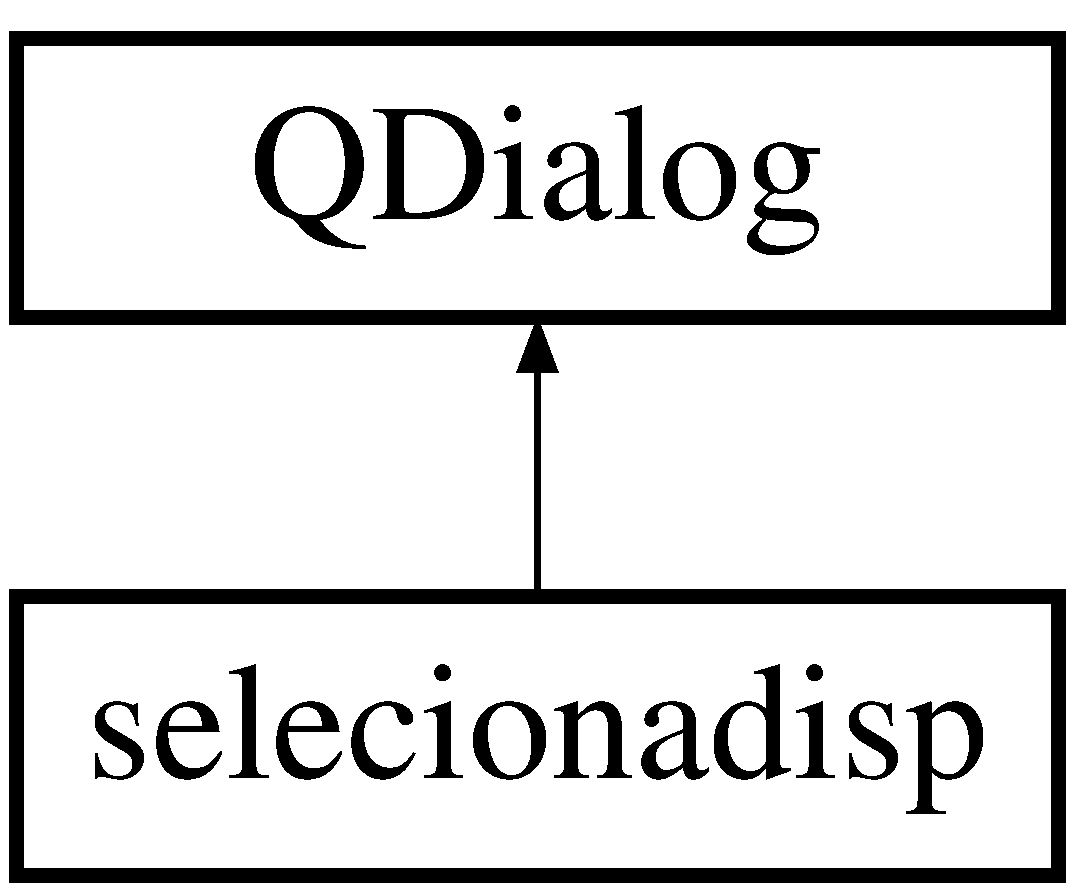
\includegraphics[height=2.000000cm]{classselecionadisp}
\end{center}
\end{figure}
\subsection*{Public Member Functions}
\begin{DoxyCompactItemize}
\item 
\hyperlink{classselecionadisp_a23cbf45ded7e90e20f7d3ea8679f856a}{selecionadisp} (Q\+Widget $\ast$parent=0)
\item 
\hyperlink{classselecionadisp_aad8dcaadb86038322f173c9b9203916e}{$\sim$selecionadisp} ()
\end{DoxyCompactItemize}


\subsection{Detailed Description}


Definition at line 10 of file selecionadisp.\+h.



\subsection{Constructor \& Destructor Documentation}
\hypertarget{classselecionadisp_a23cbf45ded7e90e20f7d3ea8679f856a}{}\label{classselecionadisp_a23cbf45ded7e90e20f7d3ea8679f856a} 
\index{selecionadisp@{selecionadisp}!selecionadisp@{selecionadisp}}
\index{selecionadisp@{selecionadisp}!selecionadisp@{selecionadisp}}
\subsubsection{\texorpdfstring{selecionadisp()}{selecionadisp()}}
{\footnotesize\ttfamily selecionadisp\+::selecionadisp (\begin{DoxyParamCaption}\item[{Q\+Widget $\ast$}]{parent = {\ttfamily 0} }\end{DoxyParamCaption})\hspace{0.3cm}{\ttfamily [explicit]}}



Definition at line 4 of file selecionadisp.\+cpp.

\hypertarget{classselecionadisp_aad8dcaadb86038322f173c9b9203916e}{}\label{classselecionadisp_aad8dcaadb86038322f173c9b9203916e} 
\index{selecionadisp@{selecionadisp}!````~selecionadisp@{$\sim$selecionadisp}}
\index{````~selecionadisp@{$\sim$selecionadisp}!selecionadisp@{selecionadisp}}
\subsubsection{\texorpdfstring{$\sim$selecionadisp()}{~selecionadisp()}}
{\footnotesize\ttfamily selecionadisp\+::$\sim$selecionadisp (\begin{DoxyParamCaption}{ }\end{DoxyParamCaption})}



Definition at line 11 of file selecionadisp.\+cpp.



The documentation for this class was generated from the following files\+:\begin{DoxyCompactItemize}
\item 
C\+:/\+Users/\+Bruno\+S\+R/\+T\+C\+C\+\_\+\+Nay\+Bru/\hyperlink{selecionadisp_8h}{selecionadisp.\+h}\item 
C\+:/\+Users/\+Bruno\+S\+R/\+T\+C\+C\+\_\+\+Nay\+Bru/\hyperlink{selecionadisp_8cpp}{selecionadisp.\+cpp}\item 
C\+:/\+Users/\+Bruno\+S\+R/\+T\+C\+C\+\_\+\+Nay\+Bru/\hyperlink{selecionaequip_8cpp}{selecionaequip.\+cpp}\end{DoxyCompactItemize}

\hypertarget{classselecionaequip}{}\section{selecionaequip Class Reference}
\label{classselecionaequip}\index{selecionaequip@{selecionaequip}}


{\ttfamily \#include $<$selecionaequip.\+h$>$}

Inheritance diagram for selecionaequip\+:\begin{figure}[H]
\begin{center}
\leavevmode
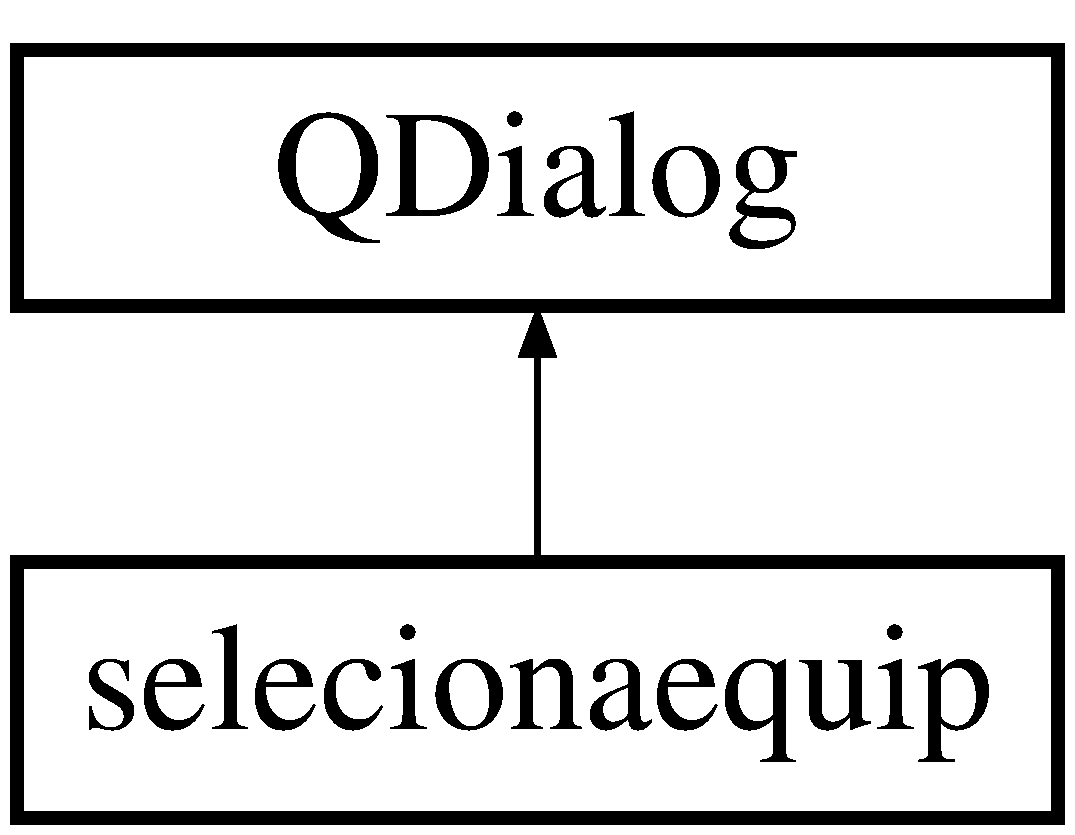
\includegraphics[height=2.000000cm]{classselecionaequip}
\end{center}
\end{figure}
\subsection*{Public Member Functions}
\begin{DoxyCompactItemize}
\item 
\hyperlink{classselecionaequip_a3ccee0d0b533a3c3d7bb53f951f022ba}{selecionaequip} (Q\+Widget $\ast$parent=0)
\item 
\hyperlink{classselecionaequip_adabd9829153adf6adb64c75a79ac7964}{$\sim$selecionaequip} ()
\end{DoxyCompactItemize}


\subsection{Detailed Description}


Definition at line 10 of file selecionaequip.\+h.



\subsection{Constructor \& Destructor Documentation}
\hypertarget{classselecionaequip_a3ccee0d0b533a3c3d7bb53f951f022ba}{}\label{classselecionaequip_a3ccee0d0b533a3c3d7bb53f951f022ba} 
\index{selecionaequip@{selecionaequip}!selecionaequip@{selecionaequip}}
\index{selecionaequip@{selecionaequip}!selecionaequip@{selecionaequip}}
\subsubsection{\texorpdfstring{selecionaequip()}{selecionaequip()}}
{\footnotesize\ttfamily selecionaequip\+::selecionaequip (\begin{DoxyParamCaption}\item[{Q\+Widget $\ast$}]{parent = {\ttfamily 0} }\end{DoxyParamCaption})\hspace{0.3cm}{\ttfamily [explicit]}}

\hypertarget{classselecionaequip_adabd9829153adf6adb64c75a79ac7964}{}\label{classselecionaequip_adabd9829153adf6adb64c75a79ac7964} 
\index{selecionaequip@{selecionaequip}!````~selecionaequip@{$\sim$selecionaequip}}
\index{````~selecionaequip@{$\sim$selecionaequip}!selecionaequip@{selecionaequip}}
\subsubsection{\texorpdfstring{$\sim$selecionaequip()}{~selecionaequip()}}
{\footnotesize\ttfamily selecionaequip\+::$\sim$selecionaequip (\begin{DoxyParamCaption}{ }\end{DoxyParamCaption})}



The documentation for this class was generated from the following file\+:\begin{DoxyCompactItemize}
\item 
C\+:/\+Users/\+Bruno\+S\+R/\+T\+C\+C\+\_\+\+Nay\+Bru/\hyperlink{selecionaequip_8h}{selecionaequip.\+h}\end{DoxyCompactItemize}

\hypertarget{class_status}{}\section{Status Class Reference}
\label{class_status}\index{Status@{Status}}


{\ttfamily \#include $<$status.\+h$>$}

\subsection*{Public Member Functions}
\begin{DoxyCompactItemize}
\item 
\hyperlink{class_status_a944586fb328a3524805748c8f7b17f32}{Status} ()
\item 
int \hyperlink{class_status_adb9c28d4221d9e2aaf9875b80b5eeaaf}{get\+Id} () const
\item 
void \hyperlink{class_status_ac2f0322cbfc1326c117eb2b244600d67}{set\+Id} (int value)
\item 
int \hyperlink{class_status_a9c4b616186e22599d7a6ce48ec724e3c}{get\+Id\+\_\+chamado} () const
\item 
void \hyperlink{class_status_aca91a7dbe10715ce9696f4b0252546ac}{set\+Id\+\_\+chamado} (int value)
\item 
Q\+String \hyperlink{class_status_a5be3ea6f3dd893039eb1278ba89d19bd}{get\+Stat} () const
\item 
void \hyperlink{class_status_aa0507ec449fc02cccb63293fed3232a4}{set\+Stat} (const Q\+String \&value)
\end{DoxyCompactItemize}


\subsection{Detailed Description}


Definition at line 9 of file status.\+h.



\subsection{Constructor \& Destructor Documentation}
\hypertarget{class_status_a944586fb328a3524805748c8f7b17f32}{}\label{class_status_a944586fb328a3524805748c8f7b17f32} 
\index{Status@{Status}!Status@{Status}}
\index{Status@{Status}!Status@{Status}}
\subsubsection{\texorpdfstring{Status()}{Status()}}
{\footnotesize\ttfamily Status\+::\+Status (\begin{DoxyParamCaption}{ }\end{DoxyParamCaption})}



Definition at line 33 of file status.\+cpp.



\subsection{Member Function Documentation}
\hypertarget{class_status_adb9c28d4221d9e2aaf9875b80b5eeaaf}{}\label{class_status_adb9c28d4221d9e2aaf9875b80b5eeaaf} 
\index{Status@{Status}!get\+Id@{get\+Id}}
\index{get\+Id@{get\+Id}!Status@{Status}}
\subsubsection{\texorpdfstring{get\+Id()}{getId()}}
{\footnotesize\ttfamily int Status\+::get\+Id (\begin{DoxyParamCaption}{ }\end{DoxyParamCaption}) const}



Definition at line 3 of file status.\+cpp.

\hypertarget{class_status_a9c4b616186e22599d7a6ce48ec724e3c}{}\label{class_status_a9c4b616186e22599d7a6ce48ec724e3c} 
\index{Status@{Status}!get\+Id\+\_\+chamado@{get\+Id\+\_\+chamado}}
\index{get\+Id\+\_\+chamado@{get\+Id\+\_\+chamado}!Status@{Status}}
\subsubsection{\texorpdfstring{get\+Id\+\_\+chamado()}{getId\_chamado()}}
{\footnotesize\ttfamily int Status\+::get\+Id\+\_\+chamado (\begin{DoxyParamCaption}{ }\end{DoxyParamCaption}) const}



Definition at line 13 of file status.\+cpp.

\hypertarget{class_status_a5be3ea6f3dd893039eb1278ba89d19bd}{}\label{class_status_a5be3ea6f3dd893039eb1278ba89d19bd} 
\index{Status@{Status}!get\+Stat@{get\+Stat}}
\index{get\+Stat@{get\+Stat}!Status@{Status}}
\subsubsection{\texorpdfstring{get\+Stat()}{getStat()}}
{\footnotesize\ttfamily Q\+String Status\+::get\+Stat (\begin{DoxyParamCaption}{ }\end{DoxyParamCaption}) const}



Definition at line 23 of file status.\+cpp.

\hypertarget{class_status_ac2f0322cbfc1326c117eb2b244600d67}{}\label{class_status_ac2f0322cbfc1326c117eb2b244600d67} 
\index{Status@{Status}!set\+Id@{set\+Id}}
\index{set\+Id@{set\+Id}!Status@{Status}}
\subsubsection{\texorpdfstring{set\+Id()}{setId()}}
{\footnotesize\ttfamily void Status\+::set\+Id (\begin{DoxyParamCaption}\item[{int}]{value }\end{DoxyParamCaption})}



Definition at line 8 of file status.\+cpp.

\hypertarget{class_status_aca91a7dbe10715ce9696f4b0252546ac}{}\label{class_status_aca91a7dbe10715ce9696f4b0252546ac} 
\index{Status@{Status}!set\+Id\+\_\+chamado@{set\+Id\+\_\+chamado}}
\index{set\+Id\+\_\+chamado@{set\+Id\+\_\+chamado}!Status@{Status}}
\subsubsection{\texorpdfstring{set\+Id\+\_\+chamado()}{setId\_chamado()}}
{\footnotesize\ttfamily void Status\+::set\+Id\+\_\+chamado (\begin{DoxyParamCaption}\item[{int}]{value }\end{DoxyParamCaption})}



Definition at line 18 of file status.\+cpp.

\hypertarget{class_status_aa0507ec449fc02cccb63293fed3232a4}{}\label{class_status_aa0507ec449fc02cccb63293fed3232a4} 
\index{Status@{Status}!set\+Stat@{set\+Stat}}
\index{set\+Stat@{set\+Stat}!Status@{Status}}
\subsubsection{\texorpdfstring{set\+Stat()}{setStat()}}
{\footnotesize\ttfamily void Status\+::set\+Stat (\begin{DoxyParamCaption}\item[{const Q\+String \&}]{value }\end{DoxyParamCaption})}



Definition at line 28 of file status.\+cpp.



The documentation for this class was generated from the following files\+:\begin{DoxyCompactItemize}
\item 
C\+:/\+Users/\+Bruno\+S\+R/\+T\+C\+C\+\_\+\+Nay\+Bru/\hyperlink{status_8h}{status.\+h}\item 
C\+:/\+Users/\+Bruno\+S\+R/\+T\+C\+C\+\_\+\+Nay\+Bru/\hyperlink{status_8cpp}{status.\+cpp}\end{DoxyCompactItemize}

\hypertarget{classtipod}{}\section{tipod Class Reference}
\label{classtipod}\index{tipod@{tipod}}


{\ttfamily \#include $<$tipod.\+h$>$}

\subsection*{Public Member Functions}
\begin{DoxyCompactItemize}
\item 
\hyperlink{classtipod_aea0583170290bcfd453f00cd7e916b26}{tipod} ()
\item 
int \hyperlink{classtipod_a8f9426cbcef23976293ae0961b382907}{get\+Id} () const
\item 
void \hyperlink{classtipod_ae3f6b8df170353ef58a862b746d3d288}{set\+Id} (int value)
\item 
Q\+String \hyperlink{classtipod_ab84c5257439bcf916770d2facad689de}{get\+Tipo} () const
\item 
void \hyperlink{classtipod_a2430c9b9e742243038b3fdb43a7bd429}{set\+Tipo} (const Q\+String \&value)
\item 
float \hyperlink{classtipod_a19cb0132a802684607abe02c0c2b63f2}{get\+S\+LA} () const
\item 
void \hyperlink{classtipod_ad0da4edb16cb79061875519e94b768d7}{set\+S\+LA} (float value)
\end{DoxyCompactItemize}


\subsection{Detailed Description}


Definition at line 7 of file tipod.\+h.



\subsection{Constructor \& Destructor Documentation}
\hypertarget{classtipod_aea0583170290bcfd453f00cd7e916b26}{}\label{classtipod_aea0583170290bcfd453f00cd7e916b26} 
\index{tipod@{tipod}!tipod@{tipod}}
\index{tipod@{tipod}!tipod@{tipod}}
\subsubsection{\texorpdfstring{tipod()}{tipod()}}
{\footnotesize\ttfamily tipod\+::tipod (\begin{DoxyParamCaption}{ }\end{DoxyParamCaption})}



Definition at line 33 of file tipod.\+cpp.



\subsection{Member Function Documentation}
\hypertarget{classtipod_a8f9426cbcef23976293ae0961b382907}{}\label{classtipod_a8f9426cbcef23976293ae0961b382907} 
\index{tipod@{tipod}!get\+Id@{get\+Id}}
\index{get\+Id@{get\+Id}!tipod@{tipod}}
\subsubsection{\texorpdfstring{get\+Id()}{getId()}}
{\footnotesize\ttfamily int tipod\+::get\+Id (\begin{DoxyParamCaption}{ }\end{DoxyParamCaption}) const}



Definition at line 3 of file tipod.\+cpp.

\hypertarget{classtipod_a19cb0132a802684607abe02c0c2b63f2}{}\label{classtipod_a19cb0132a802684607abe02c0c2b63f2} 
\index{tipod@{tipod}!get\+S\+LA@{get\+S\+LA}}
\index{get\+S\+LA@{get\+S\+LA}!tipod@{tipod}}
\subsubsection{\texorpdfstring{get\+S\+L\+A()}{getSLA()}}
{\footnotesize\ttfamily float tipod\+::get\+S\+LA (\begin{DoxyParamCaption}{ }\end{DoxyParamCaption}) const}



Definition at line 23 of file tipod.\+cpp.

\hypertarget{classtipod_ab84c5257439bcf916770d2facad689de}{}\label{classtipod_ab84c5257439bcf916770d2facad689de} 
\index{tipod@{tipod}!get\+Tipo@{get\+Tipo}}
\index{get\+Tipo@{get\+Tipo}!tipod@{tipod}}
\subsubsection{\texorpdfstring{get\+Tipo()}{getTipo()}}
{\footnotesize\ttfamily Q\+String tipod\+::get\+Tipo (\begin{DoxyParamCaption}{ }\end{DoxyParamCaption}) const}



Definition at line 13 of file tipod.\+cpp.

\hypertarget{classtipod_ae3f6b8df170353ef58a862b746d3d288}{}\label{classtipod_ae3f6b8df170353ef58a862b746d3d288} 
\index{tipod@{tipod}!set\+Id@{set\+Id}}
\index{set\+Id@{set\+Id}!tipod@{tipod}}
\subsubsection{\texorpdfstring{set\+Id()}{setId()}}
{\footnotesize\ttfamily void tipod\+::set\+Id (\begin{DoxyParamCaption}\item[{int}]{value }\end{DoxyParamCaption})}



Definition at line 8 of file tipod.\+cpp.

\hypertarget{classtipod_ad0da4edb16cb79061875519e94b768d7}{}\label{classtipod_ad0da4edb16cb79061875519e94b768d7} 
\index{tipod@{tipod}!set\+S\+LA@{set\+S\+LA}}
\index{set\+S\+LA@{set\+S\+LA}!tipod@{tipod}}
\subsubsection{\texorpdfstring{set\+S\+L\+A()}{setSLA()}}
{\footnotesize\ttfamily void tipod\+::set\+S\+LA (\begin{DoxyParamCaption}\item[{float}]{value }\end{DoxyParamCaption})}



Definition at line 28 of file tipod.\+cpp.

\hypertarget{classtipod_a2430c9b9e742243038b3fdb43a7bd429}{}\label{classtipod_a2430c9b9e742243038b3fdb43a7bd429} 
\index{tipod@{tipod}!set\+Tipo@{set\+Tipo}}
\index{set\+Tipo@{set\+Tipo}!tipod@{tipod}}
\subsubsection{\texorpdfstring{set\+Tipo()}{setTipo()}}
{\footnotesize\ttfamily void tipod\+::set\+Tipo (\begin{DoxyParamCaption}\item[{const Q\+String \&}]{value }\end{DoxyParamCaption})}



Definition at line 18 of file tipod.\+cpp.



The documentation for this class was generated from the following files\+:\begin{DoxyCompactItemize}
\item 
C\+:/\+Users/\+Bruno\+S\+R/\+T\+C\+C\+\_\+\+Nay\+Bru/\hyperlink{tipod_8h}{tipod.\+h}\item 
C\+:/\+Users/\+Bruno\+S\+R/\+T\+C\+C\+\_\+\+Nay\+Bru/\hyperlink{tipod_8cpp}{tipod.\+cpp}\end{DoxyCompactItemize}

\hypertarget{classtipo_disp}{}\section{tipo\+Disp Class Reference}
\label{classtipo_disp}\index{tipo\+Disp@{tipo\+Disp}}


{\ttfamily \#include $<$tipodisp.\+h$>$}

Inheritance diagram for tipo\+Disp\+:\begin{figure}[H]
\begin{center}
\leavevmode
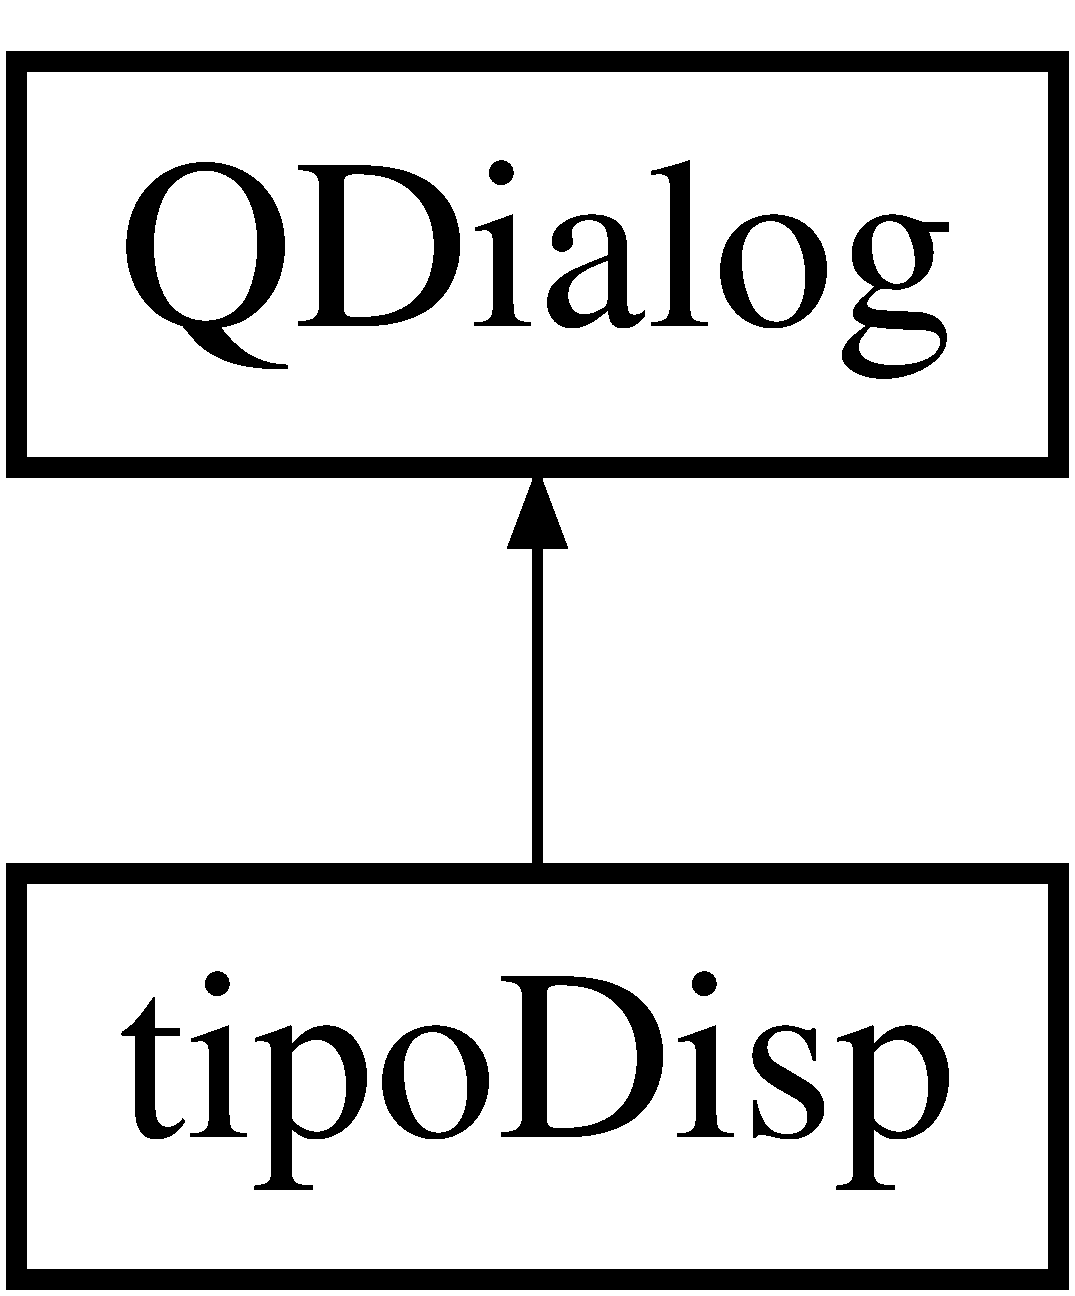
\includegraphics[height=2.000000cm]{classtipo_disp}
\end{center}
\end{figure}
\subsection*{Public Member Functions}
\begin{DoxyCompactItemize}
\item 
\hyperlink{classtipo_disp_a07b2e7bbbe94b97f3eab51ce63c30134}{tipo\+Disp} (Q\+Widget $\ast$parent=0)
\item 
\hyperlink{classtipo_disp_a235a754bbe34fe3a8fd5826e57cf3abe}{$\sim$tipo\+Disp} ()
\end{DoxyCompactItemize}


\subsection{Detailed Description}


Definition at line 10 of file tipodisp.\+h.



\subsection{Constructor \& Destructor Documentation}
\hypertarget{classtipo_disp_a07b2e7bbbe94b97f3eab51ce63c30134}{}\label{classtipo_disp_a07b2e7bbbe94b97f3eab51ce63c30134} 
\index{tipo\+Disp@{tipo\+Disp}!tipo\+Disp@{tipo\+Disp}}
\index{tipo\+Disp@{tipo\+Disp}!tipo\+Disp@{tipo\+Disp}}
\subsubsection{\texorpdfstring{tipo\+Disp()}{tipoDisp()}}
{\footnotesize\ttfamily tipo\+Disp\+::tipo\+Disp (\begin{DoxyParamCaption}\item[{Q\+Widget $\ast$}]{parent = {\ttfamily 0} }\end{DoxyParamCaption})\hspace{0.3cm}{\ttfamily [explicit]}}



Definition at line 4 of file tipodisp.\+cpp.

\hypertarget{classtipo_disp_a235a754bbe34fe3a8fd5826e57cf3abe}{}\label{classtipo_disp_a235a754bbe34fe3a8fd5826e57cf3abe} 
\index{tipo\+Disp@{tipo\+Disp}!````~tipo\+Disp@{$\sim$tipo\+Disp}}
\index{````~tipo\+Disp@{$\sim$tipo\+Disp}!tipo\+Disp@{tipo\+Disp}}
\subsubsection{\texorpdfstring{$\sim$tipo\+Disp()}{~tipoDisp()}}
{\footnotesize\ttfamily tipo\+Disp\+::$\sim$tipo\+Disp (\begin{DoxyParamCaption}{ }\end{DoxyParamCaption})}



Definition at line 11 of file tipodisp.\+cpp.



The documentation for this class was generated from the following files\+:\begin{DoxyCompactItemize}
\item 
C\+:/\+Users/\+Bruno\+S\+R/\+T\+C\+C\+\_\+\+Nay\+Bru/\hyperlink{tipodisp_8h}{tipodisp.\+h}\item 
C\+:/\+Users/\+Bruno\+S\+R/\+T\+C\+C\+\_\+\+Nay\+Bru/\hyperlink{tipodisp_8cpp}{tipodisp.\+cpp}\end{DoxyCompactItemize}

\chapter{File Documentation}
\hypertarget{cadastrochamado_8cpp}{}\section{C\+:/\+Users/\+Bruno\+S\+R/\+T\+C\+C\+\_\+\+Nay\+Bru/cadastrochamado.cpp File Reference}
\label{cadastrochamado_8cpp}\index{C\+:/\+Users/\+Bruno\+S\+R/\+T\+C\+C\+\_\+\+Nay\+Bru/cadastrochamado.\+cpp@{C\+:/\+Users/\+Bruno\+S\+R/\+T\+C\+C\+\_\+\+Nay\+Bru/cadastrochamado.\+cpp}}
{\ttfamily \#include \char`\"{}cadastrochamado.\+h\char`\"{}}\newline
{\ttfamily \#include \char`\"{}ui\+\_\+cadastrochamado.\+h\char`\"{}}\newline
{\ttfamily \#include \char`\"{}matrizraci.\+h\char`\"{}}\newline
{\ttfamily \#include \char`\"{}selecionadisp.\+h\char`\"{}}\newline

\hypertarget{cadastrochamado_8h}{}\section{C\+:/\+Users/\+Bruno\+S\+R/\+T\+C\+C\+\_\+\+Nay\+Bru/cadastrochamado.h File Reference}
\label{cadastrochamado_8h}\index{C\+:/\+Users/\+Bruno\+S\+R/\+T\+C\+C\+\_\+\+Nay\+Bru/cadastrochamado.\+h@{C\+:/\+Users/\+Bruno\+S\+R/\+T\+C\+C\+\_\+\+Nay\+Bru/cadastrochamado.\+h}}
{\ttfamily \#include $<$Q\+Widget$>$}\newline
{\ttfamily \#include $<$Q\+Table\+View$>$}\newline
{\ttfamily \#include $<$Qt\+Sql/\+Q\+Sql\+Query\+Model$>$}\newline
{\ttfamily \#include $<$Qt\+Sql/\+Q\+Sql\+Query$>$}\newline
{\ttfamily \#include $<$Qt\+Sql/\+Q\+Sql\+Table\+Model$>$}\newline
{\ttfamily \#include $<$Q\+Sql\+Database$>$}\newline
{\ttfamily \#include $<$Q\+Debug$>$}\newline
{\ttfamily \#include $<$Q\+Sql$>$}\newline
{\ttfamily \#include $<$Qt\+Core$>$}\newline
{\ttfamily \#include $<$Qt\+Gui$>$}\newline
{\ttfamily \#include $<$Q\+Sql\+Error$>$}\newline
{\ttfamily \#include $<$Q\+Message\+Box$>$}\newline
{\ttfamily \#include $<$Qt\+Sql/\+Q\+Sql\+Database$>$}\newline
{\ttfamily \#include $<$Qt\+Debug$>$}\newline
\subsection*{Classes}
\begin{DoxyCompactItemize}
\item 
class \hyperlink{classcadastrochamado}{cadastrochamado}
\end{DoxyCompactItemize}
\subsection*{Namespaces}
\begin{DoxyCompactItemize}
\item 
 \hyperlink{namespace_ui}{Ui}
\end{DoxyCompactItemize}

\hypertarget{cadastrodispositivo_8cpp}{}\section{C\+:/\+Users/\+Bruno\+S\+R/\+T\+C\+C\+\_\+\+Nay\+Bru/cadastrodispositivo.cpp File Reference}
\label{cadastrodispositivo_8cpp}\index{C\+:/\+Users/\+Bruno\+S\+R/\+T\+C\+C\+\_\+\+Nay\+Bru/cadastrodispositivo.\+cpp@{C\+:/\+Users/\+Bruno\+S\+R/\+T\+C\+C\+\_\+\+Nay\+Bru/cadastrodispositivo.\+cpp}}
{\ttfamily \#include \char`\"{}cadastrodispositivo.\+h\char`\"{}}\newline
{\ttfamily \#include \char`\"{}ui\+\_\+cadastrodispositivo.\+h\char`\"{}}\newline
{\ttfamily \#include \char`\"{}tipodisp.\+h\char`\"{}}\newline

\hypertarget{cadastrodispositivo_8h}{}\section{C\+:/\+Users/\+Bruno\+S\+R/\+T\+C\+C\+\_\+\+Nay\+Bru/cadastrodispositivo.h File Reference}
\label{cadastrodispositivo_8h}\index{C\+:/\+Users/\+Bruno\+S\+R/\+T\+C\+C\+\_\+\+Nay\+Bru/cadastrodispositivo.\+h@{C\+:/\+Users/\+Bruno\+S\+R/\+T\+C\+C\+\_\+\+Nay\+Bru/cadastrodispositivo.\+h}}
{\ttfamily \#include $<$Q\+Widget$>$}\newline
\subsection*{Classes}
\begin{DoxyCompactItemize}
\item 
class \hyperlink{classcadastrodispositivo}{cadastrodispositivo}
\end{DoxyCompactItemize}
\subsection*{Namespaces}
\begin{DoxyCompactItemize}
\item 
 \hyperlink{namespace_ui}{Ui}
\end{DoxyCompactItemize}

\hypertarget{cadastropess_8h}{}\section{C\+:/\+Users/\+Bruno\+S\+R/\+T\+C\+C\+\_\+\+Nay\+Bru/cadastropess.h File Reference}
\label{cadastropess_8h}\index{C\+:/\+Users/\+Bruno\+S\+R/\+T\+C\+C\+\_\+\+Nay\+Bru/cadastropess.\+h@{C\+:/\+Users/\+Bruno\+S\+R/\+T\+C\+C\+\_\+\+Nay\+Bru/cadastropess.\+h}}

\hypertarget{cadastropessoa_8cpp}{}\section{C\+:/\+Users/\+Bruno\+S\+R/\+T\+C\+C\+\_\+\+Nay\+Bru/cadastropessoa.cpp File Reference}
\label{cadastropessoa_8cpp}\index{C\+:/\+Users/\+Bruno\+S\+R/\+T\+C\+C\+\_\+\+Nay\+Bru/cadastropessoa.\+cpp@{C\+:/\+Users/\+Bruno\+S\+R/\+T\+C\+C\+\_\+\+Nay\+Bru/cadastropessoa.\+cpp}}
{\ttfamily \#include \char`\"{}cadastropessoa.\+h\char`\"{}}\newline
{\ttfamily \#include \char`\"{}ui\+\_\+cadastropessoa.\+h\char`\"{}}\newline
{\ttfamily \#include \char`\"{}novogrupo.\+h\char`\"{}}\newline

\hypertarget{cadastropessoa_8h}{}\section{C\+:/\+Users/\+Bruno\+S\+R/\+T\+C\+C\+\_\+\+Nay\+Bru/cadastropessoa.h File Reference}
\label{cadastropessoa_8h}\index{C\+:/\+Users/\+Bruno\+S\+R/\+T\+C\+C\+\_\+\+Nay\+Bru/cadastropessoa.\+h@{C\+:/\+Users/\+Bruno\+S\+R/\+T\+C\+C\+\_\+\+Nay\+Bru/cadastropessoa.\+h}}
{\ttfamily \#include $<$Q\+Widget$>$}\newline
\subsection*{Classes}
\begin{DoxyCompactItemize}
\item 
class \hyperlink{class_cadastropessoa}{Cadastropessoa}
\end{DoxyCompactItemize}
\subsection*{Namespaces}
\begin{DoxyCompactItemize}
\item 
 \hyperlink{namespace_ui}{Ui}
\end{DoxyCompactItemize}

\hypertarget{chamado_8cpp}{}\section{C\+:/\+Users/\+Bruno\+S\+R/\+T\+C\+C\+\_\+\+Nay\+Bru/chamado.cpp File Reference}
\label{chamado_8cpp}\index{C\+:/\+Users/\+Bruno\+S\+R/\+T\+C\+C\+\_\+\+Nay\+Bru/chamado.\+cpp@{C\+:/\+Users/\+Bruno\+S\+R/\+T\+C\+C\+\_\+\+Nay\+Bru/chamado.\+cpp}}
{\ttfamily \#include \char`\"{}chamado.\+h\char`\"{}}\newline

\hypertarget{chamado_8h}{}\section{C\+:/\+Users/\+Bruno\+S\+R/\+T\+C\+C\+\_\+\+Nay\+Bru/chamado.h File Reference}
\label{chamado_8h}\index{C\+:/\+Users/\+Bruno\+S\+R/\+T\+C\+C\+\_\+\+Nay\+Bru/chamado.\+h@{C\+:/\+Users/\+Bruno\+S\+R/\+T\+C\+C\+\_\+\+Nay\+Bru/chamado.\+h}}
{\ttfamily \#include \char`\"{}status.\+h\char`\"{}}\newline
{\ttfamily \#include \char`\"{}dispositivo.\+h\char`\"{}}\newline
{\ttfamily \#include \char`\"{}m\+\_\+raci.\+h\char`\"{}}\newline
{\ttfamily \#include $<$Q\+String$>$}\newline
\subsection*{Classes}
\begin{DoxyCompactItemize}
\item 
class \hyperlink{class_chamado}{Chamado}
\end{DoxyCompactItemize}

\hypertarget{dispositivo_8cpp}{}\section{C\+:/\+Users/\+Bruno\+S\+R/\+T\+C\+C\+\_\+\+Nay\+Bru/dispositivo.cpp File Reference}
\label{dispositivo_8cpp}\index{C\+:/\+Users/\+Bruno\+S\+R/\+T\+C\+C\+\_\+\+Nay\+Bru/dispositivo.\+cpp@{C\+:/\+Users/\+Bruno\+S\+R/\+T\+C\+C\+\_\+\+Nay\+Bru/dispositivo.\+cpp}}
{\ttfamily \#include \char`\"{}dispositivo.\+h\char`\"{}}\newline

\hypertarget{dispositivo_8h}{}\section{C\+:/\+Users/\+Bruno\+S\+R/\+T\+C\+C\+\_\+\+Nay\+Bru/dispositivo.h File Reference}
\label{dispositivo_8h}\index{C\+:/\+Users/\+Bruno\+S\+R/\+T\+C\+C\+\_\+\+Nay\+Bru/dispositivo.\+h@{C\+:/\+Users/\+Bruno\+S\+R/\+T\+C\+C\+\_\+\+Nay\+Bru/dispositivo.\+h}}
{\ttfamily \#include \char`\"{}tipod.\+h\char`\"{}}\newline
{\ttfamily \#include \char`\"{}dispositivo.\+h\char`\"{}}\newline
{\ttfamily \#include $<$Q\+String$>$}\newline
\subsection*{Classes}
\begin{DoxyCompactItemize}
\item 
class \hyperlink{class_dispositivo}{Dispositivo}
\end{DoxyCompactItemize}

\hypertarget{gerenciachamados_8cpp}{}\section{C\+:/\+Users/\+Bruno\+S\+R/\+T\+C\+C\+\_\+\+Nay\+Bru/gerenciachamados.cpp File Reference}
\label{gerenciachamados_8cpp}\index{C\+:/\+Users/\+Bruno\+S\+R/\+T\+C\+C\+\_\+\+Nay\+Bru/gerenciachamados.\+cpp@{C\+:/\+Users/\+Bruno\+S\+R/\+T\+C\+C\+\_\+\+Nay\+Bru/gerenciachamados.\+cpp}}
{\ttfamily \#include \char`\"{}gerenciachamados.\+h\char`\"{}}\newline
{\ttfamily \#include \char`\"{}ui\+\_\+gerenciachamados.\+h\char`\"{}}\newline
{\ttfamily \#include \char`\"{}cadastrochamado.\+h\char`\"{}}\newline

\hypertarget{gerenciachamados_8h}{}\section{C\+:/\+Users/\+Bruno\+S\+R/\+T\+C\+C\+\_\+\+Nay\+Bru/gerenciachamados.h File Reference}
\label{gerenciachamados_8h}\index{C\+:/\+Users/\+Bruno\+S\+R/\+T\+C\+C\+\_\+\+Nay\+Bru/gerenciachamados.\+h@{C\+:/\+Users/\+Bruno\+S\+R/\+T\+C\+C\+\_\+\+Nay\+Bru/gerenciachamados.\+h}}
{\ttfamily \#include $<$Q\+Dialog$>$}\newline
\subsection*{Classes}
\begin{DoxyCompactItemize}
\item 
class \hyperlink{classgerencia_chamados}{gerencia\+Chamados}
\end{DoxyCompactItemize}
\subsection*{Namespaces}
\begin{DoxyCompactItemize}
\item 
 \hyperlink{namespace_ui}{Ui}
\end{DoxyCompactItemize}

\hypertarget{gerenciadispositivo_8cpp}{}\section{C\+:/\+Users/\+Bruno\+S\+R/\+T\+C\+C\+\_\+\+Nay\+Bru/gerenciadispositivo.cpp File Reference}
\label{gerenciadispositivo_8cpp}\index{C\+:/\+Users/\+Bruno\+S\+R/\+T\+C\+C\+\_\+\+Nay\+Bru/gerenciadispositivo.\+cpp@{C\+:/\+Users/\+Bruno\+S\+R/\+T\+C\+C\+\_\+\+Nay\+Bru/gerenciadispositivo.\+cpp}}
{\ttfamily \#include \char`\"{}gerenciadispositivo.\+h\char`\"{}}\newline
{\ttfamily \#include \char`\"{}ui\+\_\+gerenciadispositivo.\+h\char`\"{}}\newline
{\ttfamily \#include \char`\"{}cadastrodispositivo.\+h\char`\"{}}\newline

\hypertarget{gerenciadispositivo_8h}{}\section{C\+:/\+Users/\+Bruno\+S\+R/\+T\+C\+C\+\_\+\+Nay\+Bru/gerenciadispositivo.h File Reference}
\label{gerenciadispositivo_8h}\index{C\+:/\+Users/\+Bruno\+S\+R/\+T\+C\+C\+\_\+\+Nay\+Bru/gerenciadispositivo.\+h@{C\+:/\+Users/\+Bruno\+S\+R/\+T\+C\+C\+\_\+\+Nay\+Bru/gerenciadispositivo.\+h}}
{\ttfamily \#include $<$Q\+Dialog$>$}\newline
\subsection*{Classes}
\begin{DoxyCompactItemize}
\item 
class \hyperlink{classgerencia_dispositivo}{gerencia\+Dispositivo}
\end{DoxyCompactItemize}
\subsection*{Namespaces}
\begin{DoxyCompactItemize}
\item 
 \hyperlink{namespace_ui}{Ui}
\end{DoxyCompactItemize}

\hypertarget{gerenciapessoas_8cpp}{}\section{C\+:/\+Users/\+Bruno\+S\+R/\+T\+C\+C\+\_\+\+Nay\+Bru/gerenciapessoas.cpp File Reference}
\label{gerenciapessoas_8cpp}\index{C\+:/\+Users/\+Bruno\+S\+R/\+T\+C\+C\+\_\+\+Nay\+Bru/gerenciapessoas.\+cpp@{C\+:/\+Users/\+Bruno\+S\+R/\+T\+C\+C\+\_\+\+Nay\+Bru/gerenciapessoas.\+cpp}}
{\ttfamily \#include \char`\"{}gerenciapessoas.\+h\char`\"{}}\newline
{\ttfamily \#include \char`\"{}ui\+\_\+gerenciapessoas.\+h\char`\"{}}\newline
{\ttfamily \#include \char`\"{}cadastropessoa.\+h\char`\"{}}\newline

\hypertarget{gerenciapessoas_8h}{}\section{C\+:/\+Users/\+Bruno\+S\+R/\+T\+C\+C\+\_\+\+Nay\+Bru/gerenciapessoas.h File Reference}
\label{gerenciapessoas_8h}\index{C\+:/\+Users/\+Bruno\+S\+R/\+T\+C\+C\+\_\+\+Nay\+Bru/gerenciapessoas.\+h@{C\+:/\+Users/\+Bruno\+S\+R/\+T\+C\+C\+\_\+\+Nay\+Bru/gerenciapessoas.\+h}}
{\ttfamily \#include $<$Q\+Dialog$>$}\newline
\subsection*{Classes}
\begin{DoxyCompactItemize}
\item 
class \hyperlink{classgerencia_pessoas}{gerencia\+Pessoas}
\end{DoxyCompactItemize}
\subsection*{Namespaces}
\begin{DoxyCompactItemize}
\item 
 \hyperlink{namespace_ui}{Ui}
\end{DoxyCompactItemize}

\hypertarget{grupop_8cpp}{}\section{C\+:/\+Users/\+Bruno\+S\+R/\+T\+C\+C\+\_\+\+Nay\+Bru/grupop.cpp File Reference}
\label{grupop_8cpp}\index{C\+:/\+Users/\+Bruno\+S\+R/\+T\+C\+C\+\_\+\+Nay\+Bru/grupop.\+cpp@{C\+:/\+Users/\+Bruno\+S\+R/\+T\+C\+C\+\_\+\+Nay\+Bru/grupop.\+cpp}}
{\ttfamily \#include \char`\"{}grupop.\+h\char`\"{}}\newline

\hypertarget{grupop_8h}{}\section{C\+:/\+Users/\+Bruno\+S\+R/\+T\+C\+C\+\_\+\+Nay\+Bru/grupop.h File Reference}
\label{grupop_8h}\index{C\+:/\+Users/\+Bruno\+S\+R/\+T\+C\+C\+\_\+\+Nay\+Bru/grupop.\+h@{C\+:/\+Users/\+Bruno\+S\+R/\+T\+C\+C\+\_\+\+Nay\+Bru/grupop.\+h}}
\subsection*{Classes}
\begin{DoxyCompactItemize}
\item 
class \hyperlink{class_grupo_p}{GrupoP}
\end{DoxyCompactItemize}

\hypertarget{m__raci_8cpp}{}\section{C\+:/\+Users/\+Bruno\+S\+R/\+T\+C\+C\+\_\+\+Nay\+Bru/m\+\_\+raci.cpp File Reference}
\label{m__raci_8cpp}\index{C\+:/\+Users/\+Bruno\+S\+R/\+T\+C\+C\+\_\+\+Nay\+Bru/m\+\_\+raci.\+cpp@{C\+:/\+Users/\+Bruno\+S\+R/\+T\+C\+C\+\_\+\+Nay\+Bru/m\+\_\+raci.\+cpp}}
{\ttfamily \#include \char`\"{}m\+\_\+raci.\+h\char`\"{}}\newline

\hypertarget{m__raci_8h}{}\section{C\+:/\+Users/\+Bruno\+S\+R/\+T\+C\+C\+\_\+\+Nay\+Bru/m\+\_\+raci.h File Reference}
\label{m__raci_8h}\index{C\+:/\+Users/\+Bruno\+S\+R/\+T\+C\+C\+\_\+\+Nay\+Bru/m\+\_\+raci.\+h@{C\+:/\+Users/\+Bruno\+S\+R/\+T\+C\+C\+\_\+\+Nay\+Bru/m\+\_\+raci.\+h}}
{\ttfamily \#include \char`\"{}pessoa.\+h\char`\"{}}\newline
{\ttfamily \#include \char`\"{}m\+\_\+raci.\+h\char`\"{}}\newline
\subsection*{Classes}
\begin{DoxyCompactItemize}
\item 
class \hyperlink{class_m_raci}{M\+Raci}
\end{DoxyCompactItemize}

\hypertarget{main_8cpp}{}\section{C\+:/\+Users/\+Bruno\+S\+R/\+T\+C\+C\+\_\+\+Nay\+Bru/main.cpp File Reference}
\label{main_8cpp}\index{C\+:/\+Users/\+Bruno\+S\+R/\+T\+C\+C\+\_\+\+Nay\+Bru/main.\+cpp@{C\+:/\+Users/\+Bruno\+S\+R/\+T\+C\+C\+\_\+\+Nay\+Bru/main.\+cpp}}
{\ttfamily \#include \char`\"{}mainwindow.\+h\char`\"{}}\newline
{\ttfamily \#include $<$Q\+Application$>$}\newline
\subsection*{Functions}
\begin{DoxyCompactItemize}
\item 
int \hyperlink{main_8cpp_a0ddf1224851353fc92bfbff6f499fa97}{main} (int argc, char $\ast$argv\mbox{[}$\,$\mbox{]})
\end{DoxyCompactItemize}


\subsection{Function Documentation}
\hypertarget{main_8cpp_a0ddf1224851353fc92bfbff6f499fa97}{}\label{main_8cpp_a0ddf1224851353fc92bfbff6f499fa97} 
\index{main.\+cpp@{main.\+cpp}!main@{main}}
\index{main@{main}!main.\+cpp@{main.\+cpp}}
\subsubsection{\texorpdfstring{main()}{main()}}
{\footnotesize\ttfamily int main (\begin{DoxyParamCaption}\item[{int}]{argc,  }\item[{char $\ast$}]{argv\mbox{[}$\,$\mbox{]} }\end{DoxyParamCaption})}



Definition at line 5 of file main.\+cpp.


\hypertarget{mainwindow_8cpp}{}\section{C\+:/\+Users/\+Bruno\+S\+R/\+T\+C\+C\+\_\+\+Nay\+Bru/mainwindow.cpp File Reference}
\label{mainwindow_8cpp}\index{C\+:/\+Users/\+Bruno\+S\+R/\+T\+C\+C\+\_\+\+Nay\+Bru/mainwindow.\+cpp@{C\+:/\+Users/\+Bruno\+S\+R/\+T\+C\+C\+\_\+\+Nay\+Bru/mainwindow.\+cpp}}
{\ttfamily \#include \char`\"{}mainwindow.\+h\char`\"{}}\newline
{\ttfamily \#include \char`\"{}ui\+\_\+mainwindow.\+h\char`\"{}}\newline
{\ttfamily \#include \char`\"{}gerenciapessoas.\+h\char`\"{}}\newline
{\ttfamily \#include \char`\"{}gerenciadispositivo.\+h\char`\"{}}\newline
{\ttfamily \#include \char`\"{}gerenciachamados.\+h\char`\"{}}\newline
{\ttfamily \#include \char`\"{}novogrupo.\+h\char`\"{}}\newline
{\ttfamily \#include \char`\"{}tipodisp.\+h\char`\"{}}\newline

\hypertarget{mainwindow_8h}{}\section{C\+:/\+Users/\+Bruno\+S\+R/\+T\+C\+C\+\_\+\+Nay\+Bru/mainwindow.h File Reference}
\label{mainwindow_8h}\index{C\+:/\+Users/\+Bruno\+S\+R/\+T\+C\+C\+\_\+\+Nay\+Bru/mainwindow.\+h@{C\+:/\+Users/\+Bruno\+S\+R/\+T\+C\+C\+\_\+\+Nay\+Bru/mainwindow.\+h}}
{\ttfamily \#include $<$Q\+Main\+Window$>$}\newline
{\ttfamily \#include $<$Q\+Table\+View$>$}\newline
{\ttfamily \#include $<$Qt\+Sql/\+Q\+Sql\+Query\+Model$>$}\newline
{\ttfamily \#include $<$Qt\+Sql/\+Q\+Sql\+Query$>$}\newline
{\ttfamily \#include $<$Qt\+Sql/\+Q\+Sql\+Table\+Model$>$}\newline
{\ttfamily \#include $<$Q\+Sql\+Database$>$}\newline
{\ttfamily \#include $<$Q\+Debug$>$}\newline
{\ttfamily \#include $<$Q\+Sql$>$}\newline
{\ttfamily \#include $<$Qt\+Core$>$}\newline
{\ttfamily \#include $<$Qt\+Gui$>$}\newline
{\ttfamily \#include $<$Q\+Sql\+Error$>$}\newline
{\ttfamily \#include $<$Q\+Message\+Box$>$}\newline
{\ttfamily \#include $<$Qt\+Sql/\+Q\+Sql\+Database$>$}\newline
{\ttfamily \#include $<$Qt\+Debug$>$}\newline
\subsection*{Classes}
\begin{DoxyCompactItemize}
\item 
class \hyperlink{class_main_window}{Main\+Window}
\end{DoxyCompactItemize}
\subsection*{Namespaces}
\begin{DoxyCompactItemize}
\item 
 \hyperlink{namespace_ui}{Ui}
\end{DoxyCompactItemize}

\hypertarget{matrizraci_8cpp}{}\section{C\+:/\+Users/\+Bruno\+S\+R/\+T\+C\+C\+\_\+\+Nay\+Bru/matrizraci.cpp File Reference}
\label{matrizraci_8cpp}\index{C\+:/\+Users/\+Bruno\+S\+R/\+T\+C\+C\+\_\+\+Nay\+Bru/matrizraci.\+cpp@{C\+:/\+Users/\+Bruno\+S\+R/\+T\+C\+C\+\_\+\+Nay\+Bru/matrizraci.\+cpp}}
{\ttfamily \#include \char`\"{}matrizraci.\+h\char`\"{}}\newline
{\ttfamily \#include \char`\"{}ui\+\_\+matrizraci.\+h\char`\"{}}\newline
{\ttfamily \#include $<$Q\+Message\+Box$>$}\newline
{\ttfamily \#include $<$Qt\+Sql/\+Q\+Sql\+Database$>$}\newline
{\ttfamily \#include $<$Qt\+Debug$>$}\newline
{\ttfamily \#include $<$Qt\+Sql/\+Q\+Sql\+Query\+Model$>$}\newline
{\ttfamily \#include $<$Qt\+Sql/\+Q\+Sql\+Query$>$}\newline
{\ttfamily \#include $<$Qt\+Sql/\+Q\+Sql\+Table\+Model$>$}\newline

\hypertarget{matrizraci_8h}{}\section{C\+:/\+Users/\+Bruno\+S\+R/\+T\+C\+C\+\_\+\+Nay\+Bru/matrizraci.h File Reference}
\label{matrizraci_8h}\index{C\+:/\+Users/\+Bruno\+S\+R/\+T\+C\+C\+\_\+\+Nay\+Bru/matrizraci.\+h@{C\+:/\+Users/\+Bruno\+S\+R/\+T\+C\+C\+\_\+\+Nay\+Bru/matrizraci.\+h}}
{\ttfamily \#include $<$Q\+Widget$>$}\newline
{\ttfamily \#include $<$Q\+Table\+View$>$}\newline
{\ttfamily \#include $<$Qt\+Sql/\+Q\+Sql\+Query\+Model$>$}\newline
{\ttfamily \#include $<$Qt\+Sql/\+Q\+Sql\+Query$>$}\newline
{\ttfamily \#include $<$Qt\+Sql/\+Q\+Sql\+Table\+Model$>$}\newline
{\ttfamily \#include $<$Q\+Sql\+Database$>$}\newline
{\ttfamily \#include $<$Q\+Debug$>$}\newline
{\ttfamily \#include $<$Q\+Sql$>$}\newline
{\ttfamily \#include $<$Qt\+Core$>$}\newline
{\ttfamily \#include $<$Qt\+Gui$>$}\newline
{\ttfamily \#include $<$Q\+Sql\+Error$>$}\newline
\subsection*{Classes}
\begin{DoxyCompactItemize}
\item 
class \hyperlink{classmatriz_r_a_c_i}{matriz\+R\+A\+CI}
\end{DoxyCompactItemize}
\subsection*{Namespaces}
\begin{DoxyCompactItemize}
\item 
 \hyperlink{namespace_ui}{Ui}
\end{DoxyCompactItemize}

\hypertarget{novogrupo_8cpp}{}\section{C\+:/\+Users/\+Bruno\+S\+R/\+T\+C\+C\+\_\+\+Nay\+Bru/novogrupo.cpp File Reference}
\label{novogrupo_8cpp}\index{C\+:/\+Users/\+Bruno\+S\+R/\+T\+C\+C\+\_\+\+Nay\+Bru/novogrupo.\+cpp@{C\+:/\+Users/\+Bruno\+S\+R/\+T\+C\+C\+\_\+\+Nay\+Bru/novogrupo.\+cpp}}
{\ttfamily \#include \char`\"{}novogrupo.\+h\char`\"{}}\newline
{\ttfamily \#include \char`\"{}ui\+\_\+novogrupo.\+h\char`\"{}}\newline

\hypertarget{novogrupo_8h}{}\section{C\+:/\+Users/\+Bruno\+S\+R/\+T\+C\+C\+\_\+\+Nay\+Bru/novogrupo.h File Reference}
\label{novogrupo_8h}\index{C\+:/\+Users/\+Bruno\+S\+R/\+T\+C\+C\+\_\+\+Nay\+Bru/novogrupo.\+h@{C\+:/\+Users/\+Bruno\+S\+R/\+T\+C\+C\+\_\+\+Nay\+Bru/novogrupo.\+h}}
{\ttfamily \#include $<$Q\+Widget$>$}\newline
\subsection*{Classes}
\begin{DoxyCompactItemize}
\item 
class \hyperlink{classnovo_grupo}{novo\+Grupo}
\end{DoxyCompactItemize}
\subsection*{Namespaces}
\begin{DoxyCompactItemize}
\item 
 \hyperlink{namespace_ui}{Ui}
\end{DoxyCompactItemize}

\hypertarget{pessoa_8cpp}{}\section{C\+:/\+Users/\+Bruno\+S\+R/\+T\+C\+C\+\_\+\+Nay\+Bru/pessoa.cpp File Reference}
\label{pessoa_8cpp}\index{C\+:/\+Users/\+Bruno\+S\+R/\+T\+C\+C\+\_\+\+Nay\+Bru/pessoa.\+cpp@{C\+:/\+Users/\+Bruno\+S\+R/\+T\+C\+C\+\_\+\+Nay\+Bru/pessoa.\+cpp}}
{\ttfamily \#include \char`\"{}pessoa.\+h\char`\"{}}\newline

\hypertarget{pessoa_8h}{}\section{C\+:/\+Users/\+Bruno\+S\+R/\+T\+C\+C\+\_\+\+Nay\+Bru/pessoa.h File Reference}
\label{pessoa_8h}\index{C\+:/\+Users/\+Bruno\+S\+R/\+T\+C\+C\+\_\+\+Nay\+Bru/pessoa.\+h@{C\+:/\+Users/\+Bruno\+S\+R/\+T\+C\+C\+\_\+\+Nay\+Bru/pessoa.\+h}}
{\ttfamily \#include $<$string$>$}\newline
\subsection*{Classes}
\begin{DoxyCompactItemize}
\item 
class \hyperlink{classpessoa}{pessoa}
\end{DoxyCompactItemize}

\hypertarget{selecionadisp_8cpp}{}\section{C\+:/\+Users/\+Bruno\+S\+R/\+T\+C\+C\+\_\+\+Nay\+Bru/selecionadisp.cpp File Reference}
\label{selecionadisp_8cpp}\index{C\+:/\+Users/\+Bruno\+S\+R/\+T\+C\+C\+\_\+\+Nay\+Bru/selecionadisp.\+cpp@{C\+:/\+Users/\+Bruno\+S\+R/\+T\+C\+C\+\_\+\+Nay\+Bru/selecionadisp.\+cpp}}
{\ttfamily \#include \char`\"{}selecionadisp.\+h\char`\"{}}\newline
{\ttfamily \#include \char`\"{}ui\+\_\+selecionadisp.\+h\char`\"{}}\newline

\hypertarget{selecionadisp_8h}{}\section{C\+:/\+Users/\+Bruno\+S\+R/\+T\+C\+C\+\_\+\+Nay\+Bru/selecionadisp.h File Reference}
\label{selecionadisp_8h}\index{C\+:/\+Users/\+Bruno\+S\+R/\+T\+C\+C\+\_\+\+Nay\+Bru/selecionadisp.\+h@{C\+:/\+Users/\+Bruno\+S\+R/\+T\+C\+C\+\_\+\+Nay\+Bru/selecionadisp.\+h}}
{\ttfamily \#include $<$Q\+Dialog$>$}\newline
\subsection*{Classes}
\begin{DoxyCompactItemize}
\item 
class \hyperlink{classselecionadisp}{selecionadisp}
\end{DoxyCompactItemize}
\subsection*{Namespaces}
\begin{DoxyCompactItemize}
\item 
 \hyperlink{namespace_ui}{Ui}
\end{DoxyCompactItemize}

\hypertarget{selecionaequip_8cpp}{}\section{C\+:/\+Users/\+Bruno\+S\+R/\+T\+C\+C\+\_\+\+Nay\+Bru/selecionaequip.cpp File Reference}
\label{selecionaequip_8cpp}\index{C\+:/\+Users/\+Bruno\+S\+R/\+T\+C\+C\+\_\+\+Nay\+Bru/selecionaequip.\+cpp@{C\+:/\+Users/\+Bruno\+S\+R/\+T\+C\+C\+\_\+\+Nay\+Bru/selecionaequip.\+cpp}}
{\ttfamily \#include \char`\"{}selecionaequip.\+h\char`\"{}}\newline
{\ttfamily \#include \char`\"{}ui\+\_\+selecionaequip.\+h\char`\"{}}\newline

\hypertarget{selecionaequip_8h}{}\section{C\+:/\+Users/\+Bruno\+S\+R/\+T\+C\+C\+\_\+\+Nay\+Bru/selecionaequip.h File Reference}
\label{selecionaequip_8h}\index{C\+:/\+Users/\+Bruno\+S\+R/\+T\+C\+C\+\_\+\+Nay\+Bru/selecionaequip.\+h@{C\+:/\+Users/\+Bruno\+S\+R/\+T\+C\+C\+\_\+\+Nay\+Bru/selecionaequip.\+h}}
{\ttfamily \#include $<$Q\+Dialog$>$}\newline
\subsection*{Classes}
\begin{DoxyCompactItemize}
\item 
class \hyperlink{classselecionaequip}{selecionaequip}
\end{DoxyCompactItemize}
\subsection*{Namespaces}
\begin{DoxyCompactItemize}
\item 
 \hyperlink{namespace_ui}{Ui}
\end{DoxyCompactItemize}

\hypertarget{status_8cpp}{}\section{C\+:/\+Users/\+Bruno\+S\+R/\+T\+C\+C\+\_\+\+Nay\+Bru/status.cpp File Reference}
\label{status_8cpp}\index{C\+:/\+Users/\+Bruno\+S\+R/\+T\+C\+C\+\_\+\+Nay\+Bru/status.\+cpp@{C\+:/\+Users/\+Bruno\+S\+R/\+T\+C\+C\+\_\+\+Nay\+Bru/status.\+cpp}}
{\ttfamily \#include \char`\"{}status.\+h\char`\"{}}\newline

\hypertarget{status_8h}{}\section{C\+:/\+Users/\+Bruno\+S\+R/\+T\+C\+C\+\_\+\+Nay\+Bru/status.h File Reference}
\label{status_8h}\index{C\+:/\+Users/\+Bruno\+S\+R/\+T\+C\+C\+\_\+\+Nay\+Bru/status.\+h@{C\+:/\+Users/\+Bruno\+S\+R/\+T\+C\+C\+\_\+\+Nay\+Bru/status.\+h}}
{\ttfamily \#include \char`\"{}status.\+h\char`\"{}}\newline
{\ttfamily \#include $<$Q\+String$>$}\newline
\subsection*{Classes}
\begin{DoxyCompactItemize}
\item 
class \hyperlink{class_status}{Status}
\end{DoxyCompactItemize}

\hypertarget{tipod_8cpp}{}\section{C\+:/\+Users/\+Bruno\+S\+R/\+T\+C\+C\+\_\+\+Nay\+Bru/tipod.cpp File Reference}
\label{tipod_8cpp}\index{C\+:/\+Users/\+Bruno\+S\+R/\+T\+C\+C\+\_\+\+Nay\+Bru/tipod.\+cpp@{C\+:/\+Users/\+Bruno\+S\+R/\+T\+C\+C\+\_\+\+Nay\+Bru/tipod.\+cpp}}
{\ttfamily \#include \char`\"{}tipod.\+h\char`\"{}}\newline

\hypertarget{tipod_8h}{}\section{C\+:/\+Users/\+Bruno\+S\+R/\+T\+C\+C\+\_\+\+Nay\+Bru/tipod.h File Reference}
\label{tipod_8h}\index{C\+:/\+Users/\+Bruno\+S\+R/\+T\+C\+C\+\_\+\+Nay\+Bru/tipod.\+h@{C\+:/\+Users/\+Bruno\+S\+R/\+T\+C\+C\+\_\+\+Nay\+Bru/tipod.\+h}}
{\ttfamily \#include $<$Q\+String$>$}\newline
\subsection*{Classes}
\begin{DoxyCompactItemize}
\item 
class \hyperlink{classtipod}{tipod}
\end{DoxyCompactItemize}

\hypertarget{tipodisp_8cpp}{}\section{C\+:/\+Users/\+Bruno\+S\+R/\+T\+C\+C\+\_\+\+Nay\+Bru/tipodisp.cpp File Reference}
\label{tipodisp_8cpp}\index{C\+:/\+Users/\+Bruno\+S\+R/\+T\+C\+C\+\_\+\+Nay\+Bru/tipodisp.\+cpp@{C\+:/\+Users/\+Bruno\+S\+R/\+T\+C\+C\+\_\+\+Nay\+Bru/tipodisp.\+cpp}}
{\ttfamily \#include \char`\"{}tipodisp.\+h\char`\"{}}\newline
{\ttfamily \#include \char`\"{}ui\+\_\+tipodisp.\+h\char`\"{}}\newline

\hypertarget{tipodisp_8h}{}\section{C\+:/\+Users/\+Bruno\+S\+R/\+T\+C\+C\+\_\+\+Nay\+Bru/tipodisp.h File Reference}
\label{tipodisp_8h}\index{C\+:/\+Users/\+Bruno\+S\+R/\+T\+C\+C\+\_\+\+Nay\+Bru/tipodisp.\+h@{C\+:/\+Users/\+Bruno\+S\+R/\+T\+C\+C\+\_\+\+Nay\+Bru/tipodisp.\+h}}
{\ttfamily \#include $<$Q\+Dialog$>$}\newline
\subsection*{Classes}
\begin{DoxyCompactItemize}
\item 
class \hyperlink{classtipo_disp}{tipo\+Disp}
\end{DoxyCompactItemize}
\subsection*{Namespaces}
\begin{DoxyCompactItemize}
\item 
 \hyperlink{namespace_ui}{Ui}
\end{DoxyCompactItemize}

%--- End generated contents ---

% Index
\backmatter
\newpage
\phantomsection
\clearemptydoublepage
\addcontentsline{toc}{chapter}{Index}
\printindex

\end{document}
